\section{RF analysis}

At each session's end, a RF analysis was held to assess whether the V1 imaged position corresponded to neurons with RFs centered in the center of the visual field, as these were the fixed intended positions for the subsequent SM spatial structure analysis.

Responses of each ROI were baseline subtracted and analysed trial by trial, mapping each trial's response to the visual field position that the corresponding stimulus was presented at (figure \ref{rfanalysis}, left panels).

Then, these responses were averaged over repetition trials, portraying mean response levels for each of the visual field positions (figure \ref{rfanalysis}, middle panels).

Finally, normalized gray-scale maps were produced for the response maps $R(az, el)$, with $az$ and $el$ the azimuth and elevation retinotopic coordinates, averaging over time on each of the positions' mean trace responses (figure \ref{rfanalysis}, right panels).

\begin{figure}[H] \centering 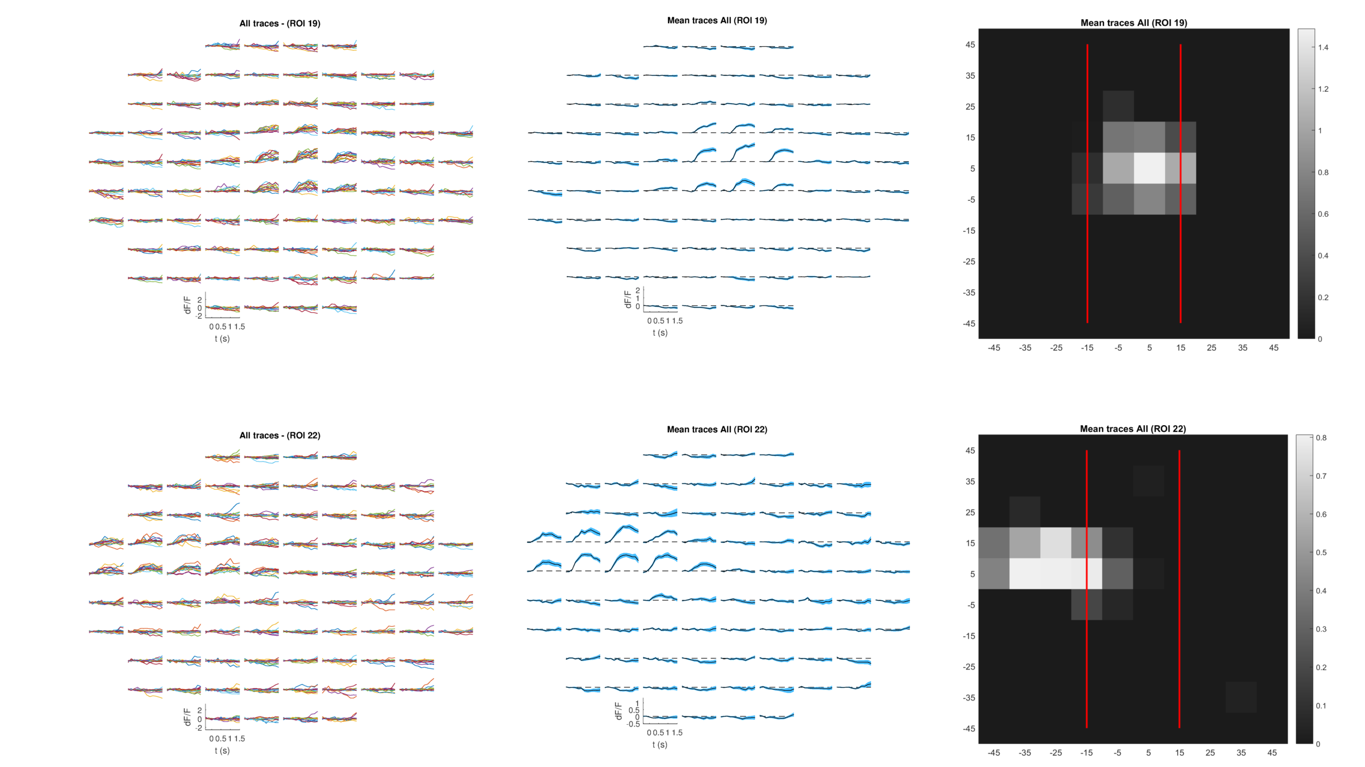
\includegraphics[width=13cm,height=13cm,keepaspectratio]{Figures/7.Results/rf/rfs.png} 
\caption{Example receptive field measurements for two different cells. On the left, each of the 14 trial-type repetition trace response is represented in a different colour, for each of the visual field stimulated region. On the middle column, the mean traces, averaging over the 14 repetitions are represented also for each azimuth and elevation center stimulus condition. The right column represents the relative response strengths to each of the stimulus positions, in a gray-scale colour map.
\newline \textbf{Top:} Example cell with well centred RF.
\textbf{Bottom:} Example cell with RF center in the left portion of the visual field.}
\label{rfanalysis}
\end{figure}

Each of these neurons' response maps was fitted to 2D-Gaussian ellipses, using Matlab implementation of the least-squares Levenberg-Marquardt algorithm (as in \cite{Marques2018}):

\begin{dmath}
R(az,el)=a+b\times \exp \left[ - \left( \dfrac{az-az_0}\times \cos(\theta)+ el-el_0)\times \sin(\theta){\sqrt{2} \times \sigma_1}\right)^2 - \left( \dfrac{-(az-az_0) \times sin \theta + (el-el_0)\times \cos(\theta)}{\sqrt{2} \times \sigma_2}\right)^2\right]
\end{dmath}

with $(az_0, el_0)$ the 2D Gaussian center coordinates, $\sigma_1$ and $\sigma_2$ the standard deviations of the gaussian across the two dimensions, $\theta$ the rotation angle between the gaussian and the $(az,el)$ axis, $a$ an offset parameter and $b$ an amplitude parameter.

The RF was then defined as the ellipse centred at $(az_0, ele_0)$ and limited by the standard deviations  ($\sigma_1$, $\sigma_2$):

\begin{equation}
\left[ \left( \dfrac{(az-az_0)\cdot \cos(\theta) + (el-el_0)\cdot \sin(\theta)}{\sigma_1}\right)^2 + \left(\dfrac{-(az-az_0)\cdot \sin(\theta) + (el-el_0)\cdot \cos(\theta)}{\sigma_2}\right)^2\right]=1
\end{equation}

The subsequent analysis was restricted to fits with $R^2>0.5$, as lower values corresponded to RF unreliable estimations. Within 10 sessions with 4 planes each, across 4 animals, 3168 out of 4198 dataset ROIs ($75\%$) were considered.

Analysing plane by plane, for each animal and session (example planes in figure \ref{ellipses}), one could assess that most of the considered RF centers were placed with similar centers within the retinotopical space, as theoretically expected for the short distances of $200 \times 200) \mu m$ imaged V1 planes. 

Two of the sessions showed very high elevation RFs, and were thus discarded for subsequent analysis, leaving 2772 measured RF cells and a total of 3728 cells ($74\%$ fitted RFs) to be analysed in regards to SM effects.

\begin{figure}[H] \centering 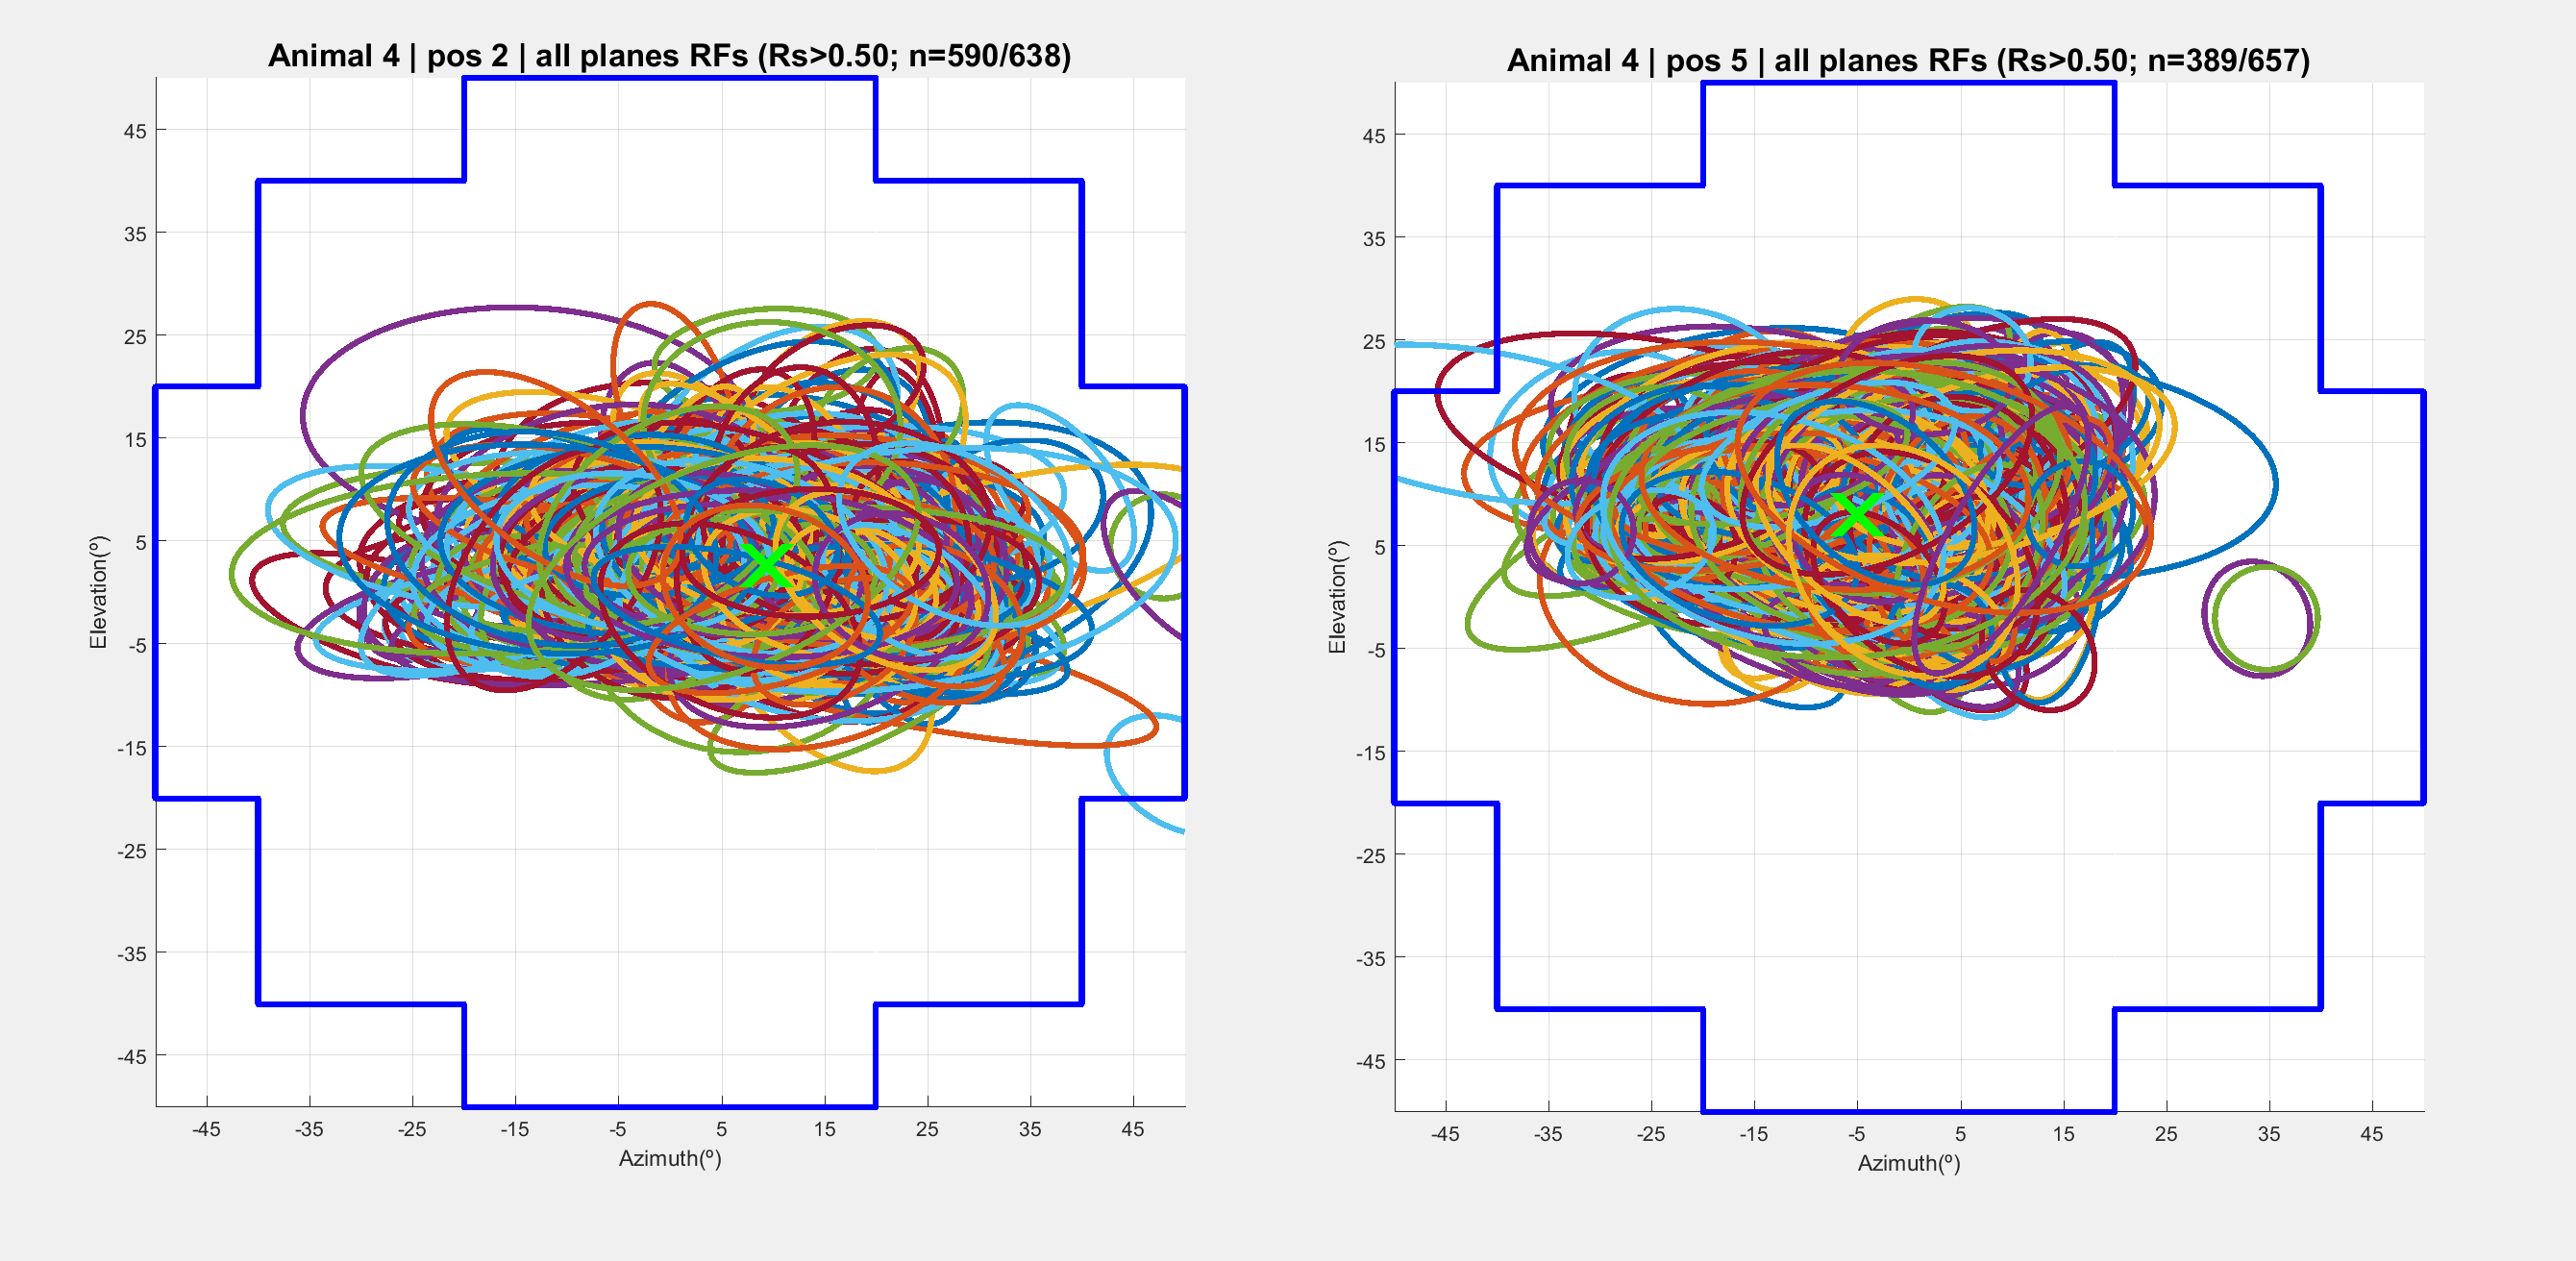
\includegraphics[width=13cm,height=13cm,keepaspectratio]{Figures/7.Results/rf/ellipsesAnimal4pos2andpos5.png} 
\caption{Superimposed 2D gaussian ellipsoidal fits for each neuron in the same plane. Two planes from two different animals are presented as examples.}
\label{ellipses}
\end{figure}

\section{Tuning analysis}

To validate bpod's tuning protocol, the selected neurons were analysed in regards to their direction (8 directions), spatial (2) and temporal (2) frequencies tuning selectivity.

Neurons in V1 can have orientation selectivity (\cite{Hubel1959}, \cite{Hubel1962}), that is, respond more strongly to a preferred orientation than to any other orientation. For mice, these orientation-selective (OS) cells are not organized into functional columns as they are for carnivores and primates (\cite{Hubel1962}, \cite{Hubel1968}), yet they do present strong orientation selectivity (\cite{Girman1999}, \cite{Ohki2005}). 

Moreover, a subset of  OS cells are also direction-selective (DS): these respond most strongly to a preferred direction than to any other.

For orientation analysis, responses of opposite directions are averaged together, and ploted on polar coordinates (figures \ref{tuninganalysisOS} and \ref{tuninganalysisDS}). The vector sum of responses at each individual trial (combining the trials for each of the same orientation opposed directions) then forms the \textit{orientation vector} of that trial. The orientation vectors for all trials then exhibit the cell's orientation tuning properties.
In the analogous way, for direction analysis, each trial measurement is binned to different direction labels, and the vector sum of the responses at individual directions then amounts to a direction vector for each trial. Direction vectors for all trials represent the cell's direction tuning properties.

Statistical significance is assessed with vector-based Hotelling's $t^2$-tests with confidence of 95\% in this project's case, as suggested by examinations in \cite{Mazurek2014}, to ask whether the 2D mean of the distribution of orientation and or direction vectors differ from (0,0).
 
 For any orientation, if the responses to a given orientation are significantly higher than responses to any other orientation, then the former is called the neuron's preferred orientation. This differential effect can be measured with an orientation selectivity index (OSI), for the preferred orientation response in the considered space. With  $R_{pref_or}$ the responses to the preferred orientation and $R_{orth}$ the responses to the orientation orthogonal to the preferred:
\begin{equation}
\text{OSI}= \dfrac{R_{pref_or} - R_{orth}}{R_{pref_or} + R_{orth}}
\end{equation}

Similarly, in the direction space, a preferred direction can also be determined for neurons that have significantly higher responses in one direction than they do in the null direction relative to the former. A DSI can be computed, for the direction doublet:

\begin{equation}
\text{DSI}=\dfrac{R_{pref} - R_{null}}{R_{pref} + R_{null}}
\end{equation}

In regards to the spatial and frequency tuning, here we used a restricted $(2 \times 2)$ space and found as expected (\cite{Whichpapershowsthis?}) that for most cells, in this space, the preferred spatial frequency was of 0.04 cycles per degree and the preferred temporal frequency was at 1 Hz.

Here, we present two example cell responses for the different stimulus conditions in the tuning protocol: an OS cell (figure \ref{tuninganalysisDS}) and a DS cell (figure \ref{tuninganalysisOS}).

\begin{figure}[H] \centering 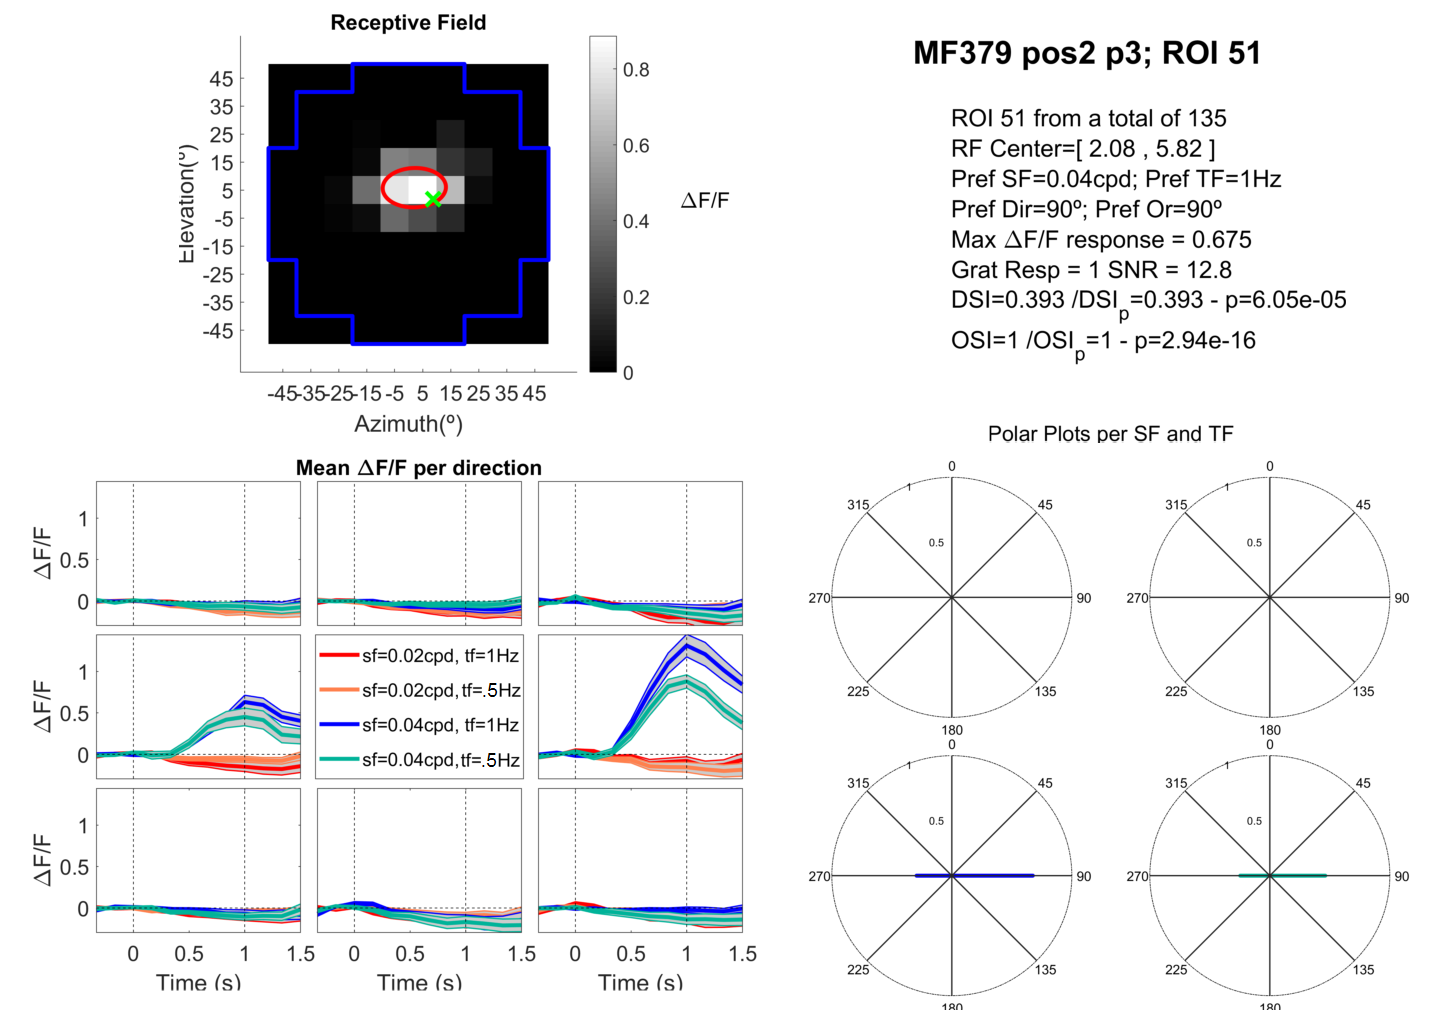
\includegraphics[width=12cm,height=12cm,keepaspectratio]{Figures/7.Results/tuning/MF379_pos2_p3_ROI0051.png} 
%\caption{rf Positions all}
\label{tuninganalysisOS}
\end{figure}

\begin{figure}[H] \centering 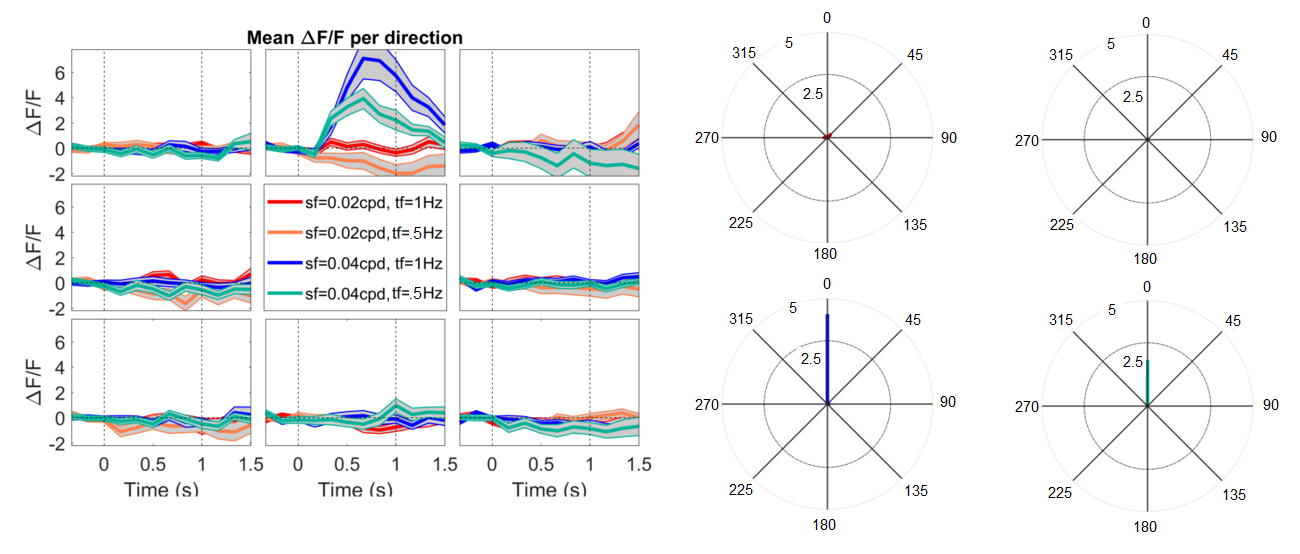
\includegraphics[width=12.5cm,height=12.5cm,keepaspectratio]{Figures/7.Results/tuning/CM006_pos1_p4_ROI0138.png} 
%\caption{rf Positions all}
\label{tuninganalysisDS}
\end{figure}

\section{SM analysis - individual cells}
\subsection{DS example cell}


\begin{figure}[H] \centering 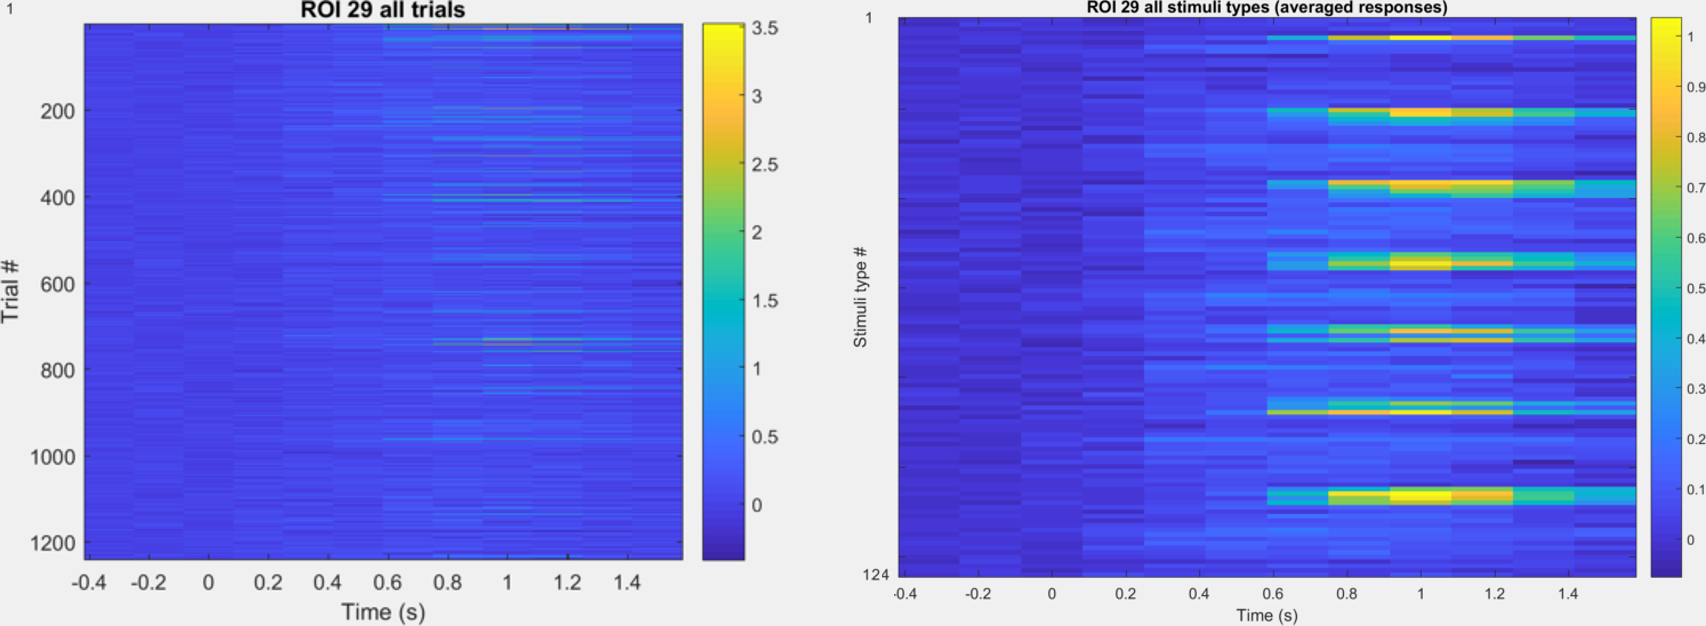
\includegraphics[width=12.5cm,height=12.5cm,keepaspectratio]{Figures/7.Results/individualSM/roi 29 mf379 pos5/roi29.png} 
%\caption{rf Positions all}
\end{figure}

\begin{figure}[H] \centering 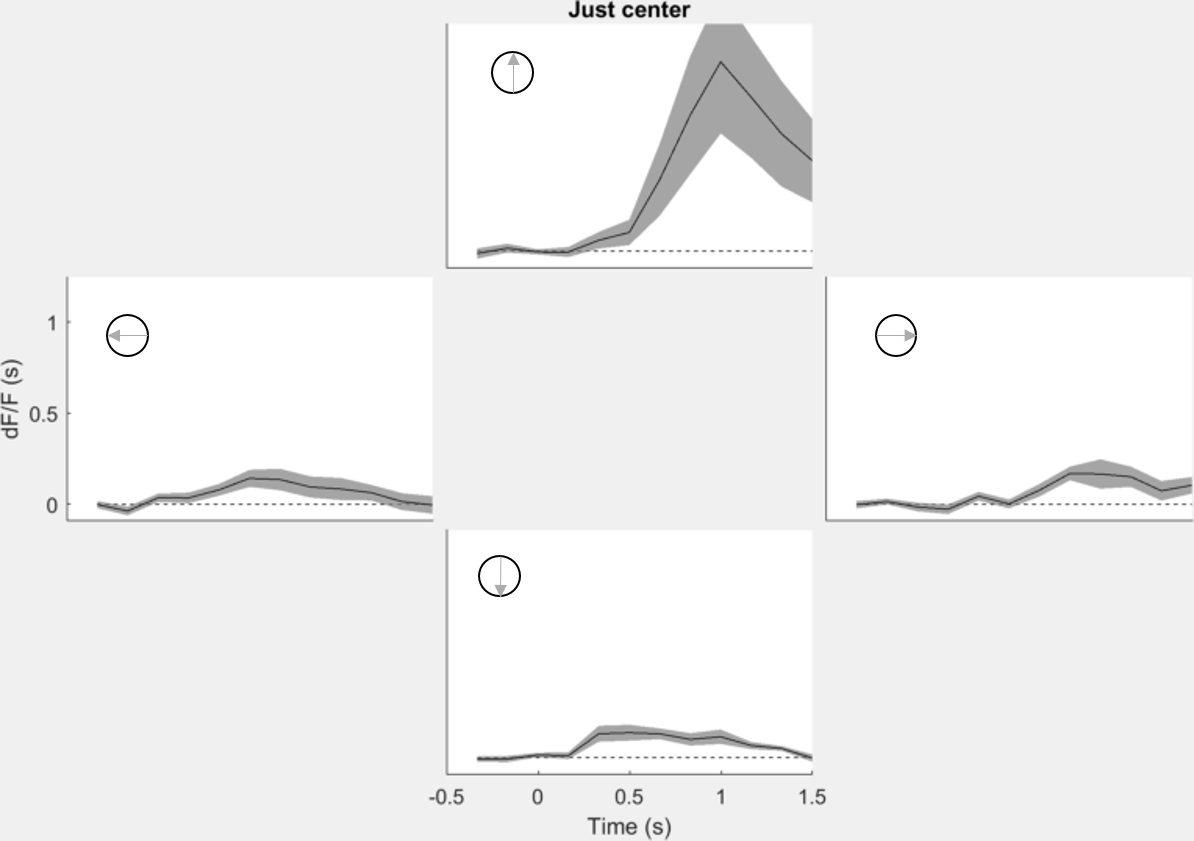
\includegraphics[width=12.5cm,height=12.5cm,keepaspectratio]{Figures/7.Results/individualSM/roi 29 mf379 pos5/justcenter.png} 
%\caption{rf Positions all}
\end{figure}

\begin{figure}[H] \centering 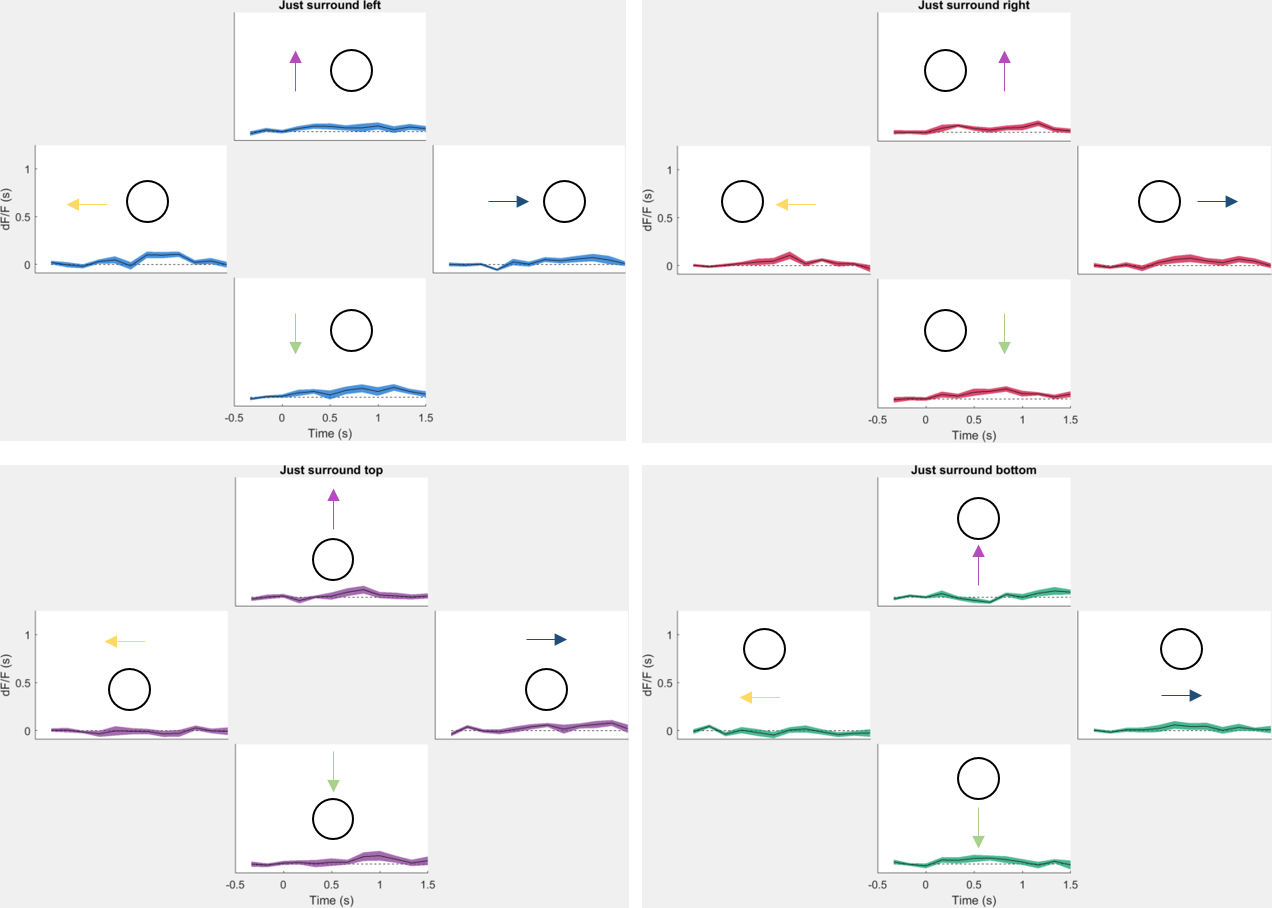
\includegraphics[width=12.5cm,height=12.5cm,keepaspectratio]{Figures/7.Results/individualSM/roi 29 mf379 pos5/justsurrscol.png} 
%\caption{rf Positions all}
\end{figure}

\begin{figure}[H] \centering 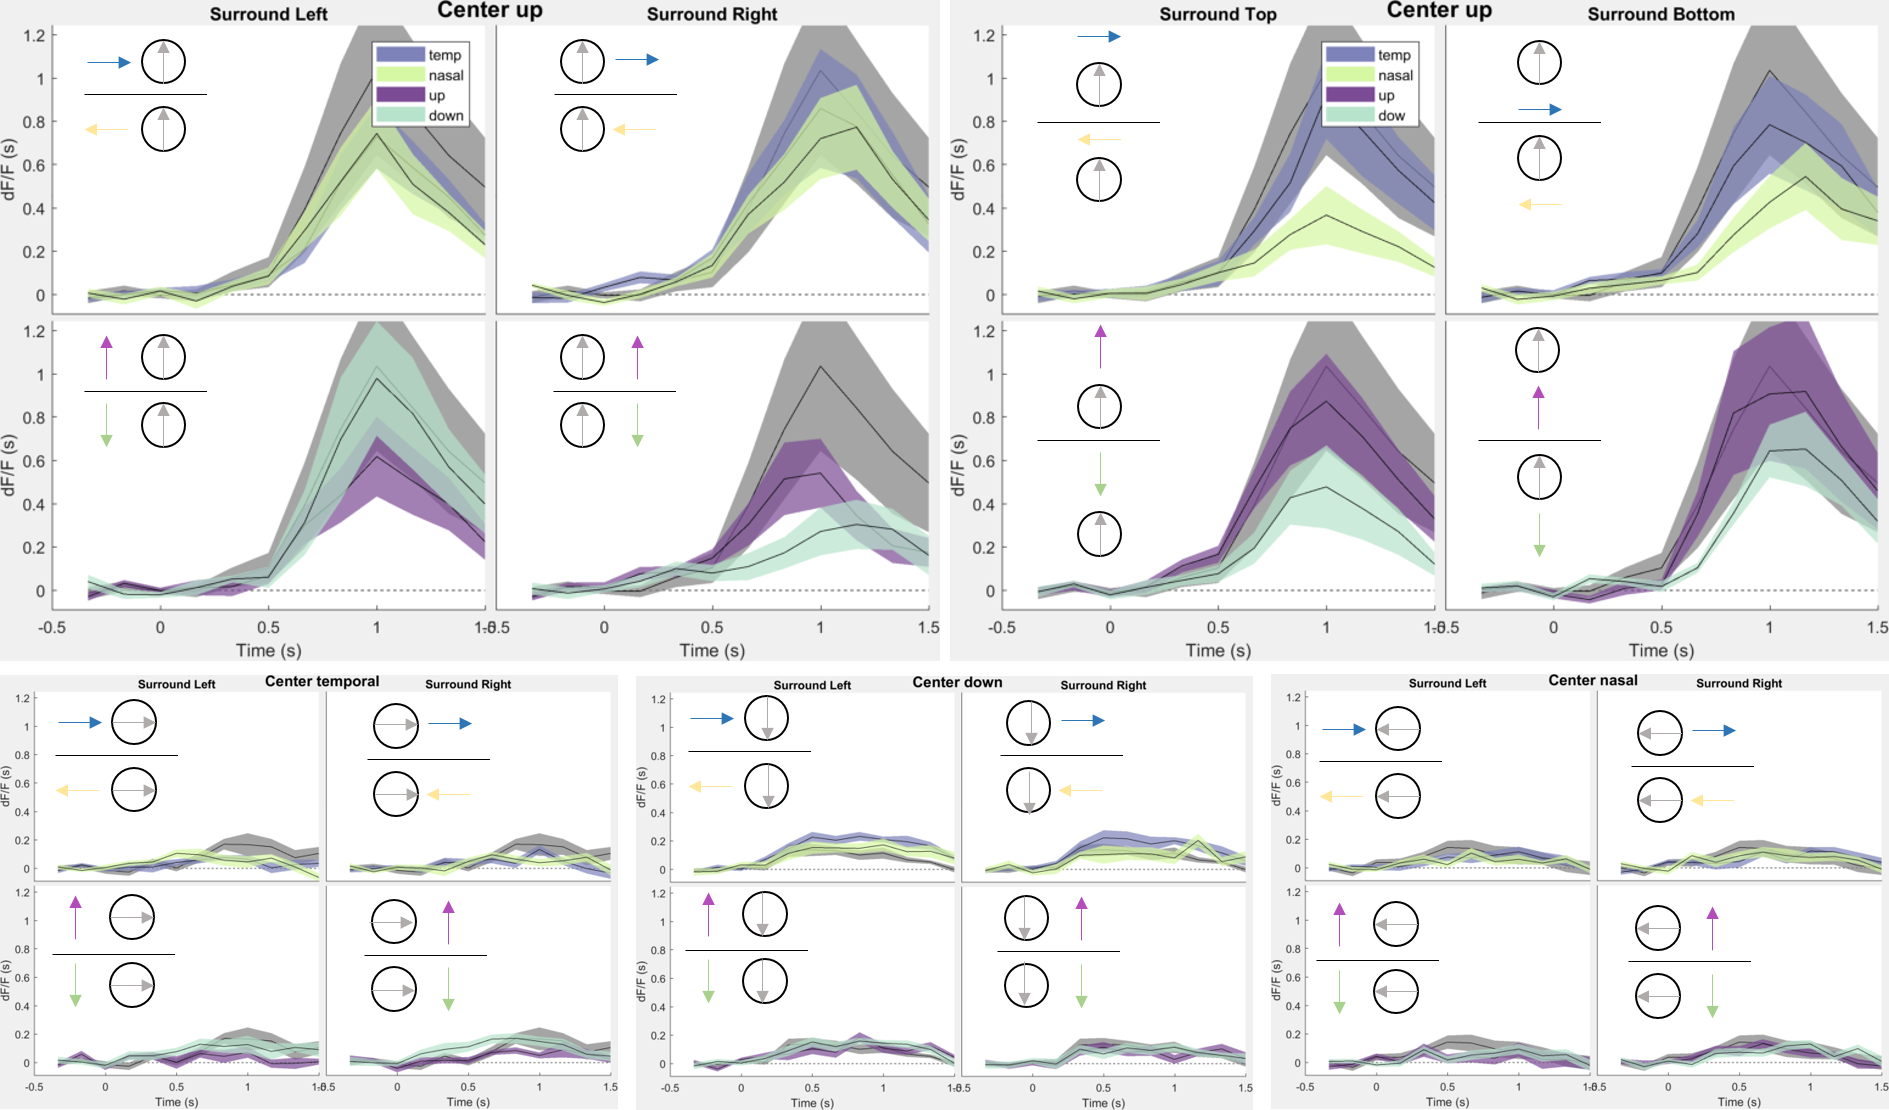
\includegraphics[width=14cm,height=12.5cm,keepaspectratio]{Figures/7.Results/individualSM/roi 29 mf379 pos5/surroundresponses.png} 
%\caption{rf Positions all}
\end{figure}

\begin{figure}[H] \centering 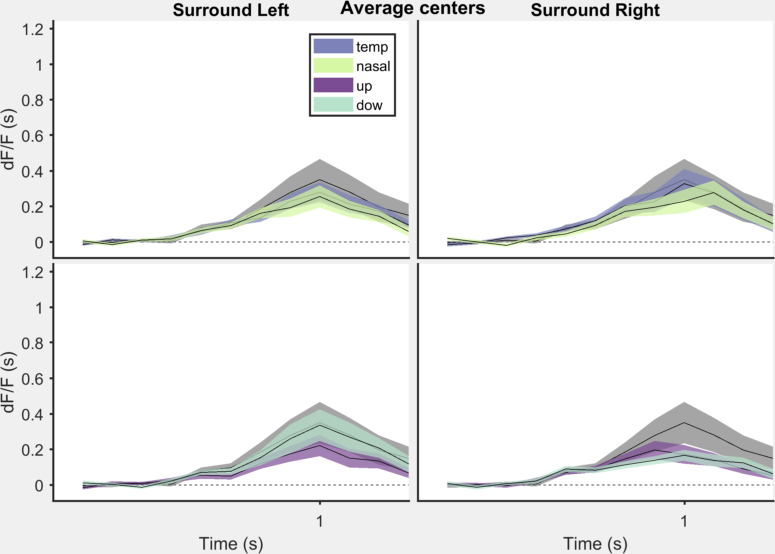
\includegraphics[width=12.5cm,height=12.5cm,keepaspectratio]{Figures/7.Results/individualSM/roi 29 mf379 pos5/averagecenters.png} 
%\caption{rf Positions all}
\end{figure}

\subsection{OS example cell}

\begin{figure}[H] \centering 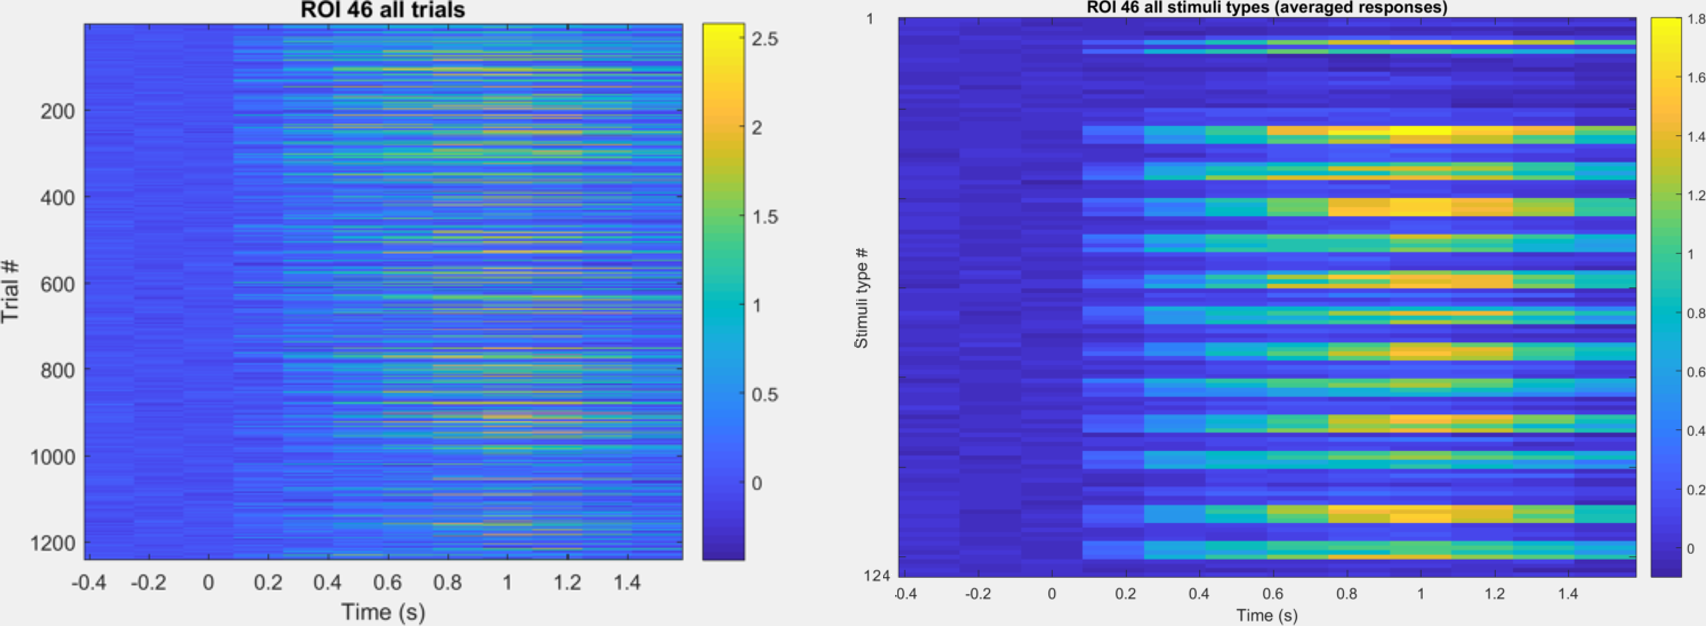
\includegraphics[width=12.5cm,height=12.5cm,keepaspectratio]{Figures/7.Results/individualSM/roi 46 mf379 pos2/roi46.png} 
%\caption{rf Positions all}
\end{figure}

\begin{figure}[H] \centering 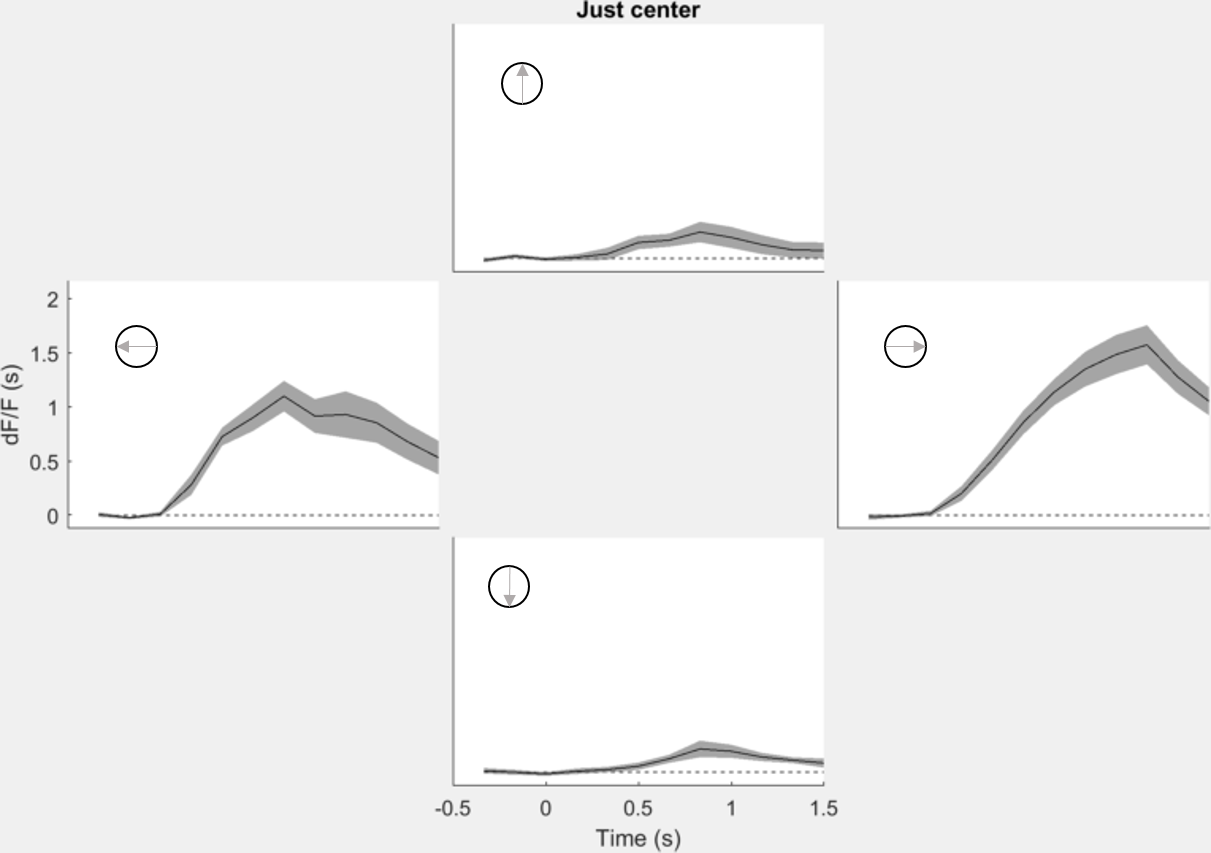
\includegraphics[width=12.5cm,height=12.5cm,keepaspectratio]{Figures/7.Results/individualSM/roi 46 mf379 pos2/center.png} 
%\caption{rf Positions all}
\end{figure}

\begin{figure}[H] \centering 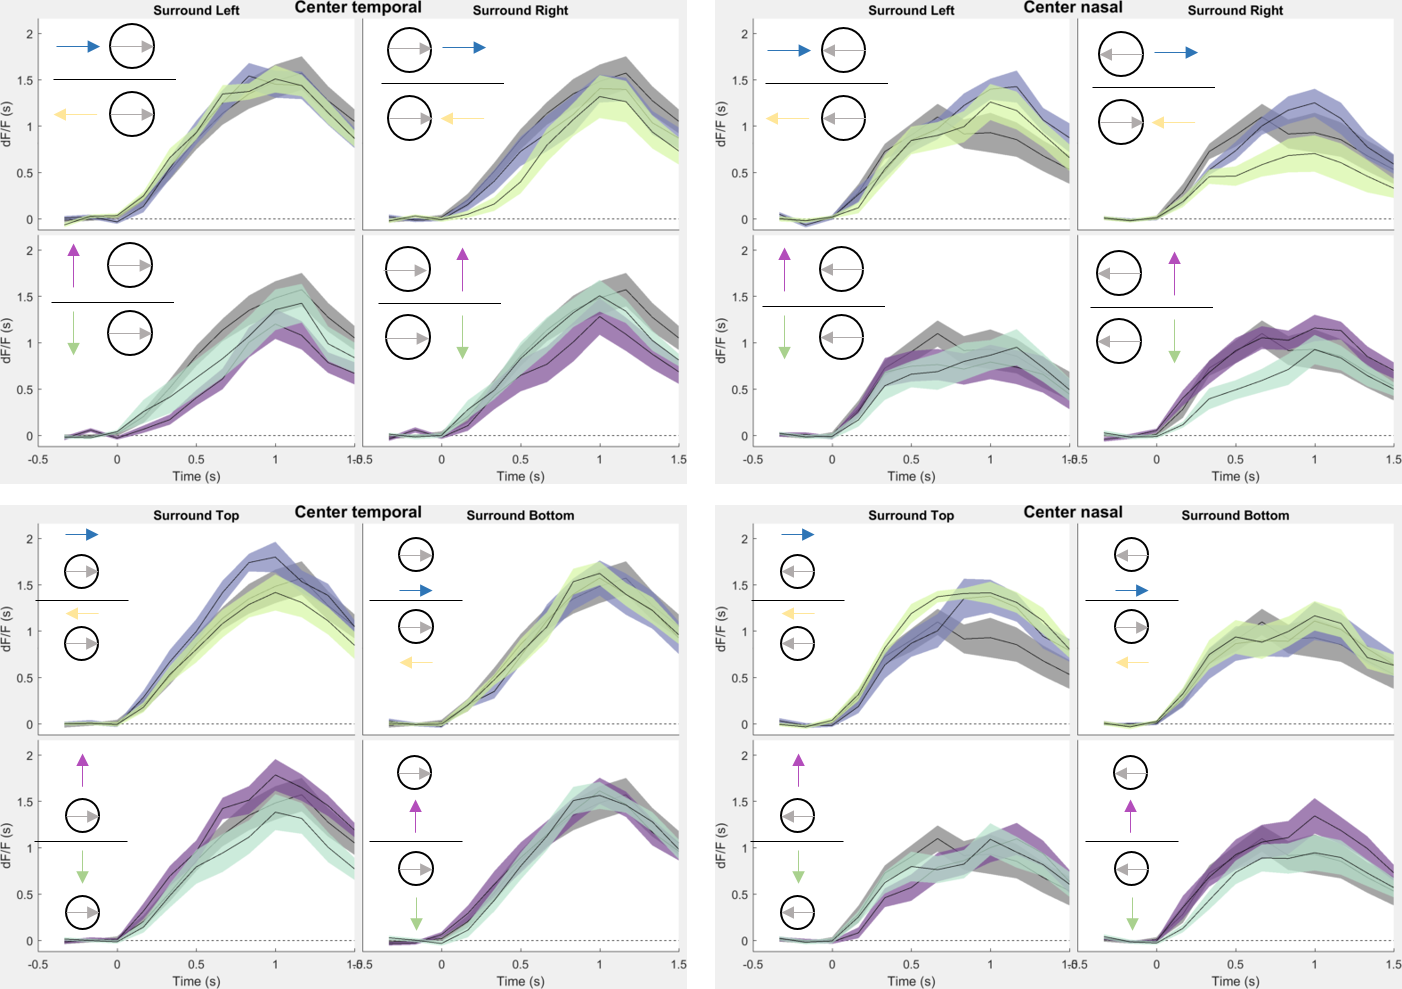
\includegraphics[width=12.5cm,height=12.5cm,keepaspectratio]{Figures/7.Results/individualSM/roi 46 mf379 pos2/surrs.png} 
%\caption{rf Positions all}
\end{figure}

\section{SM analysis - cell population}

\subsection{Data ROI groups}

\begin{figure}[H] \centering \includegraphics[width=5cm,height=5cm,keepaspectratio]{Figures/7.Results/data/ROIvisualCenter.png} 
%\caption{rf Positions all}
\end{figure}

\begin{figure}[H] \centering 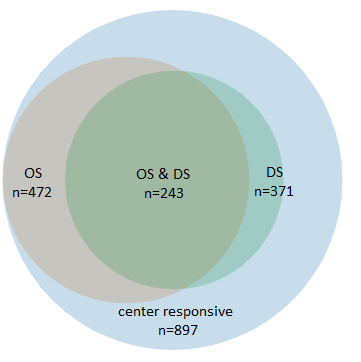
\includegraphics[width=5cm,height=5cm,keepaspectratio]{Figures/7.Results/data/centerOSDS.png} 
%\caption{rf Positions all}
\end{figure}

\begin{figure}[H] \centering 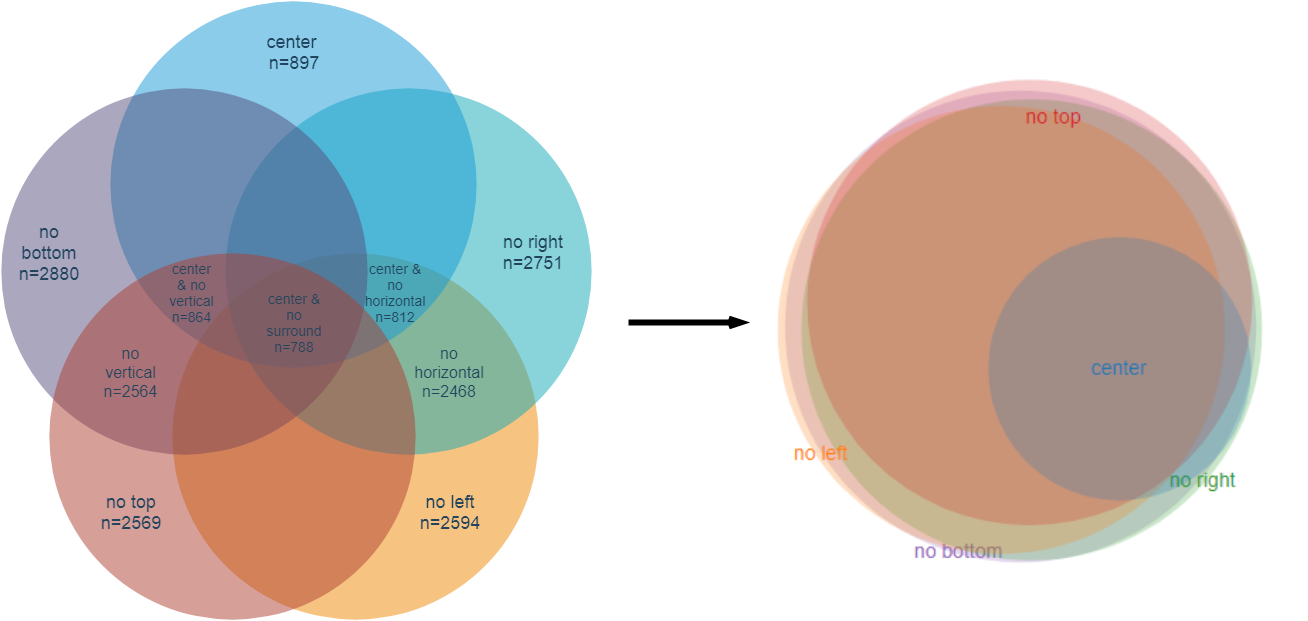
\includegraphics[width=15cm,height=15cm,keepaspectratio]{Figures/7.Results/data/SMdata.png} 
%\caption{rf Positions all}
\end{figure}

\subsection{RF center positions and SM protocol center-only: all population and per animal}

\begin{figure}[H] \centering 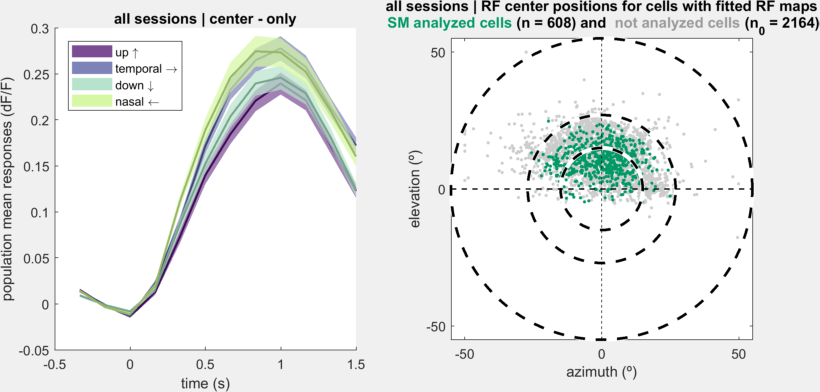
\includegraphics[width=12cm,height=12cm,keepaspectratio]{Figures/7.Results/population/sel/1_popPlots_rfPositions.png} 
%\caption{rf Positions all}
\end{figure}

%\begin{figure}[H] \centering 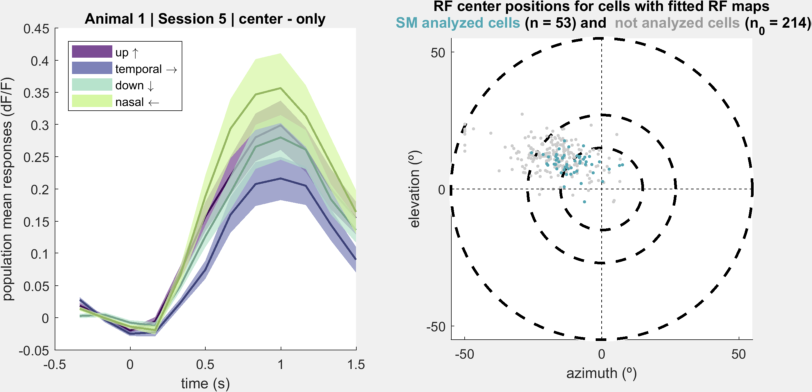
\includegraphics[width=12cm,height=12cm,keepaspectratio]{Figures/7.Results/population/sel/2_popPlots_Animal1_Session5.png} 
%%\caption{2 popPlots Animal1 Session5.} 
%\end{figure}

%\begin{figure}[H] \centering 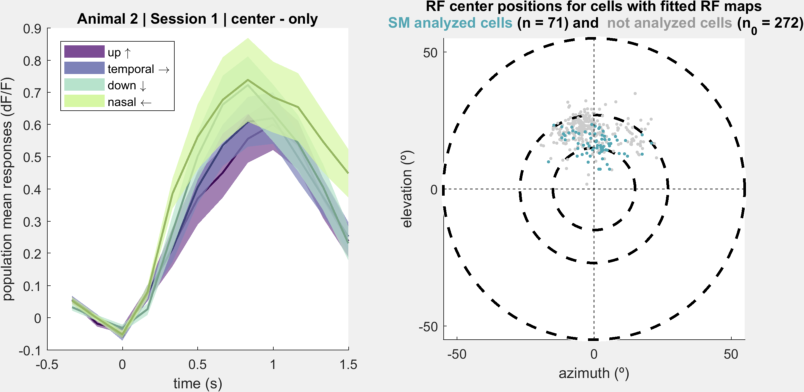
\includegraphics[width=12cm,height=12cm,keepaspectratio]{Figures/7.Results/population/sel/3_popPlots_Animal2_Session1.png} 
%%\caption{3 popPlots Animal2 Session1.} 
%\end{figure}
%
%\begin{figure}[H] \centering 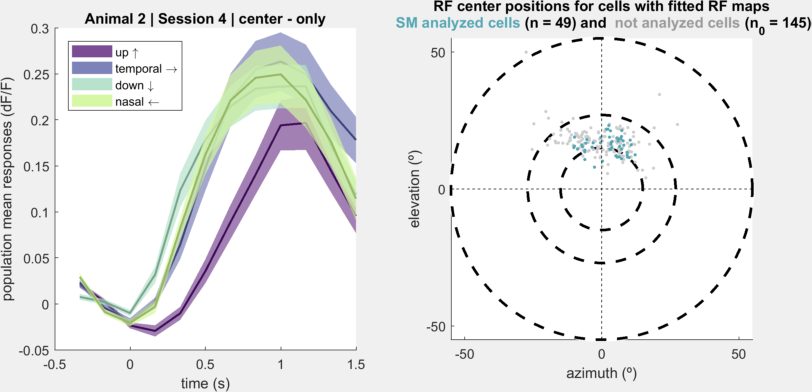
\includegraphics[width=13cm,height=13cm,keepaspectratio]{Figures/7.Results/population/sel/4_popPlots_Animal2_Session4.png} 
%%\caption{4 popPlots Animal2 Session4} 
%\end{figure}
%
%\begin{figure}[H] \centering 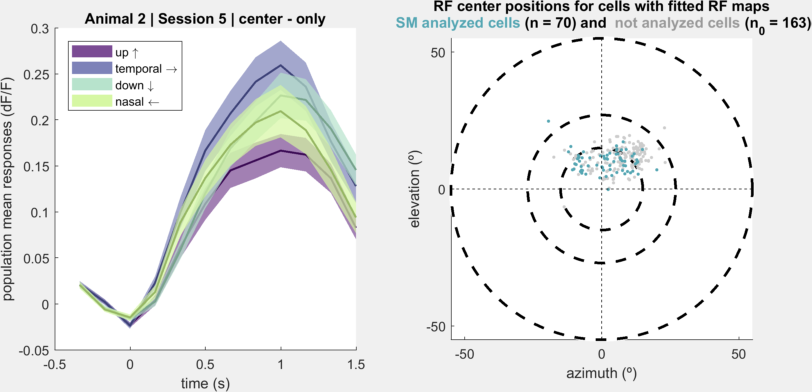
\includegraphics[width=13cm,height=13cm,keepaspectratio]{Figures/7.Results/population/sel/5_popPlots_Animal2_Session5.png} 
%%\caption{5_popPlots_Animal2_Session5} 
%\end{figure}

\begin{figure}[H] \centering 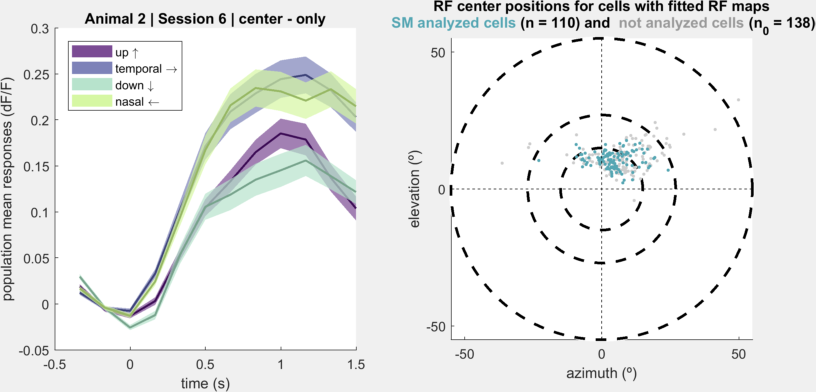
\includegraphics[width=13cm,height=13cm,keepaspectratio]{Figures/7.Results/population/sel/6_popPlots_Animal2_Session6.png} 
%\caption{6_popPlots_Animal2_Session6} 
\end{figure}

%\begin{figure}[H] \centering 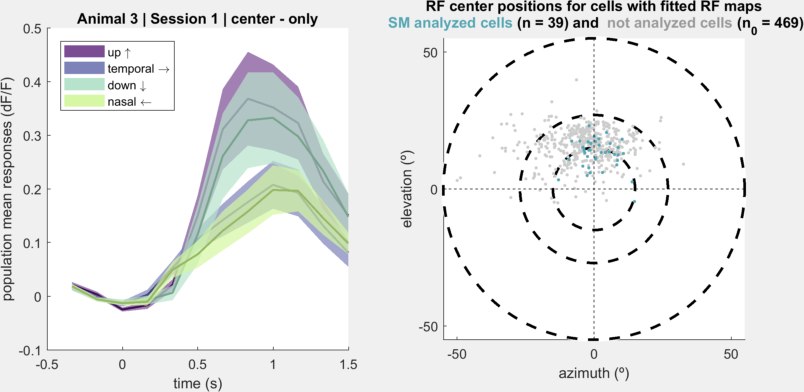
\includegraphics[width=13cm,height=13cm,keepaspectratio]{Figures/7.Results/population/sel/7_popPlots_Animal3_Session1.png} 
%%\caption{7_popPlots_Animal3_Session1} 
%\end{figure}
%
%\begin{figure}[H] \centering 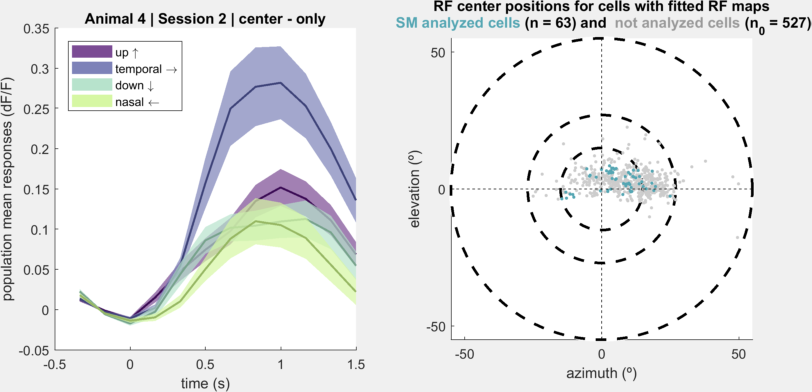
\includegraphics[width=13cm,height=13cm,keepaspectratio]{Figures/7.Results/population/sel/8_popPlots_Animal4_Session2.png} 
%%\caption{8_popPlots_Animal4_Session2} 
%\end{figure}
%
%\begin{figure}[H] \centering 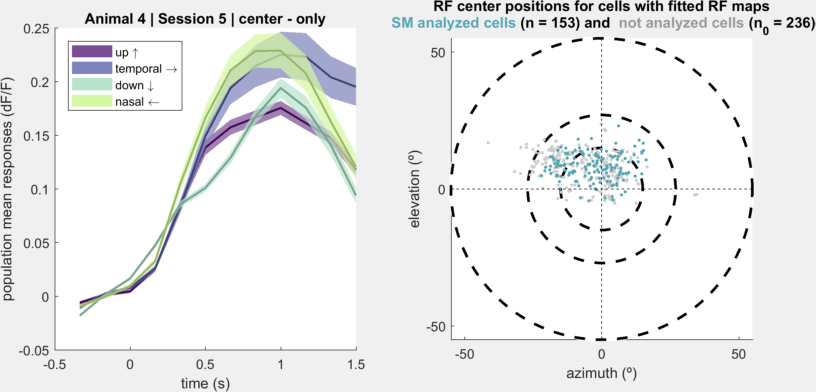
\includegraphics[width=13cm,height=13cm,keepaspectratio]{Figures/7.Results/population/sel/9_popPlots_Animal4_Session5.png} 
%%\caption{9_popPlots_Animal4_Session5} 
%\end{figure}

\begin{figure}[H] \centering 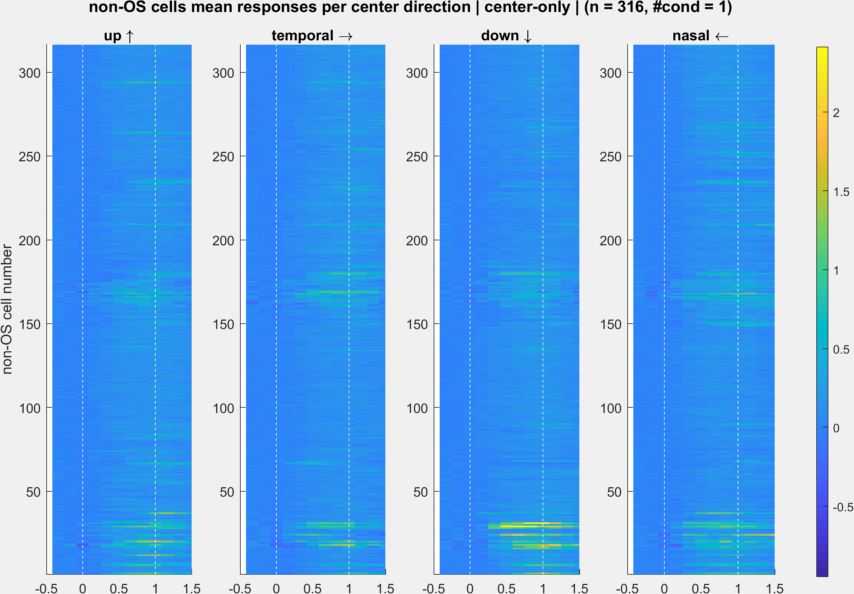
\includegraphics[width=11cm,height=11cm,keepaspectratio]{Figures/7.Results/population/sel/10_popPlots_nonOS_centerOnly.png} 
%\caption{10_popPlots_nonOS_centerOnly} 
\end{figure}

\begin{figure}[H] \centering 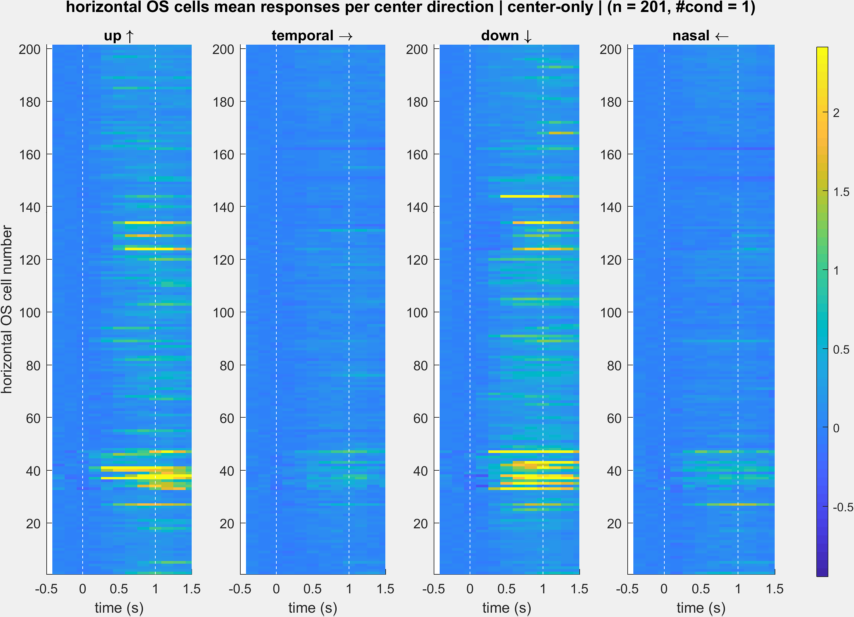
\includegraphics[width=11cm,height=11cm,keepaspectratio]{Figures/7.Results/population/sel/11_popPlots_horzOS_centerOnly.png} 
%\caption{11_popPlots_horzOS_centerOnly} 
\end{figure}

\begin{figure}[H] \centering 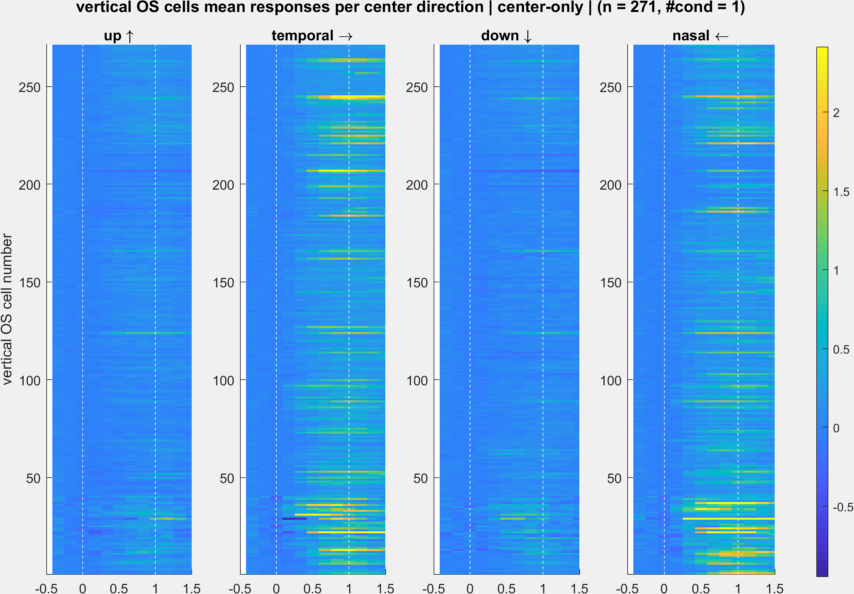
\includegraphics[width=11cm,height=11cm,keepaspectratio]{Figures/7.Results/population/sel/12_popPlots_vertOS_centerOnly.png} 
%\caption{12_popPlots_vertOS_centerOnly} 
\end{figure}

\subsection{Comparisons between conditions}

\subsubsection{Surround number effect}

\begin{figure}[H] \centering 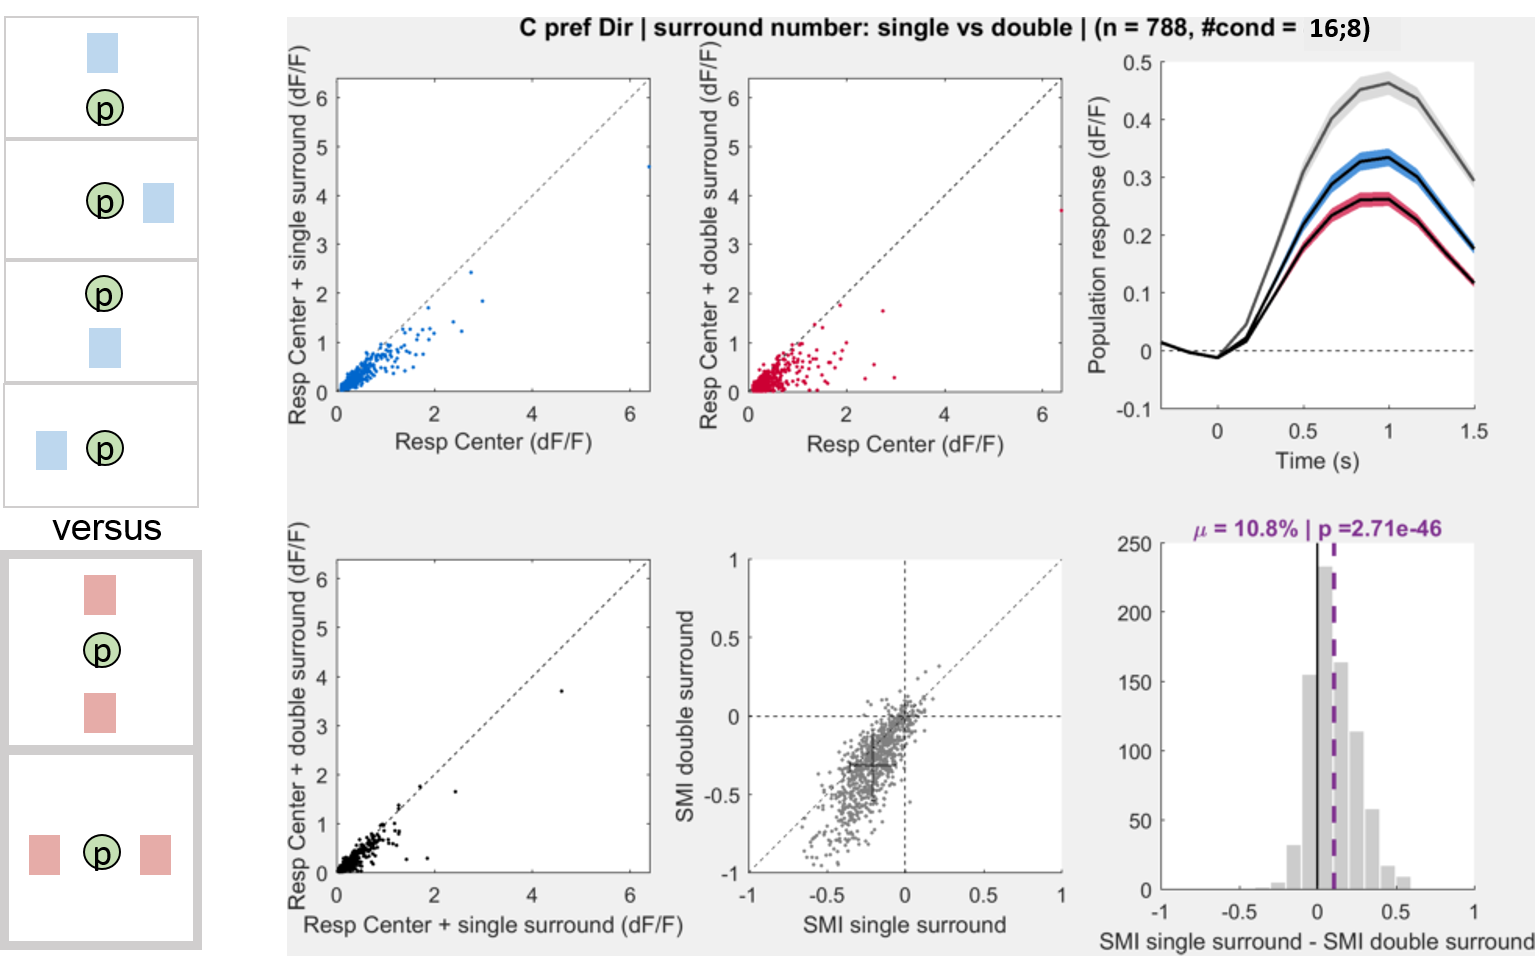
\includegraphics[width=11cm,height=11cm,keepaspectratio]{Figures/7.Results/population/sel/diagrams/1.png} 
%\caption{13_popPlots_VisROIs_CprefDir_Snumber} 
\end{figure}

\subsubsection{Surround position effect}

\begin{figure}[H] \centering 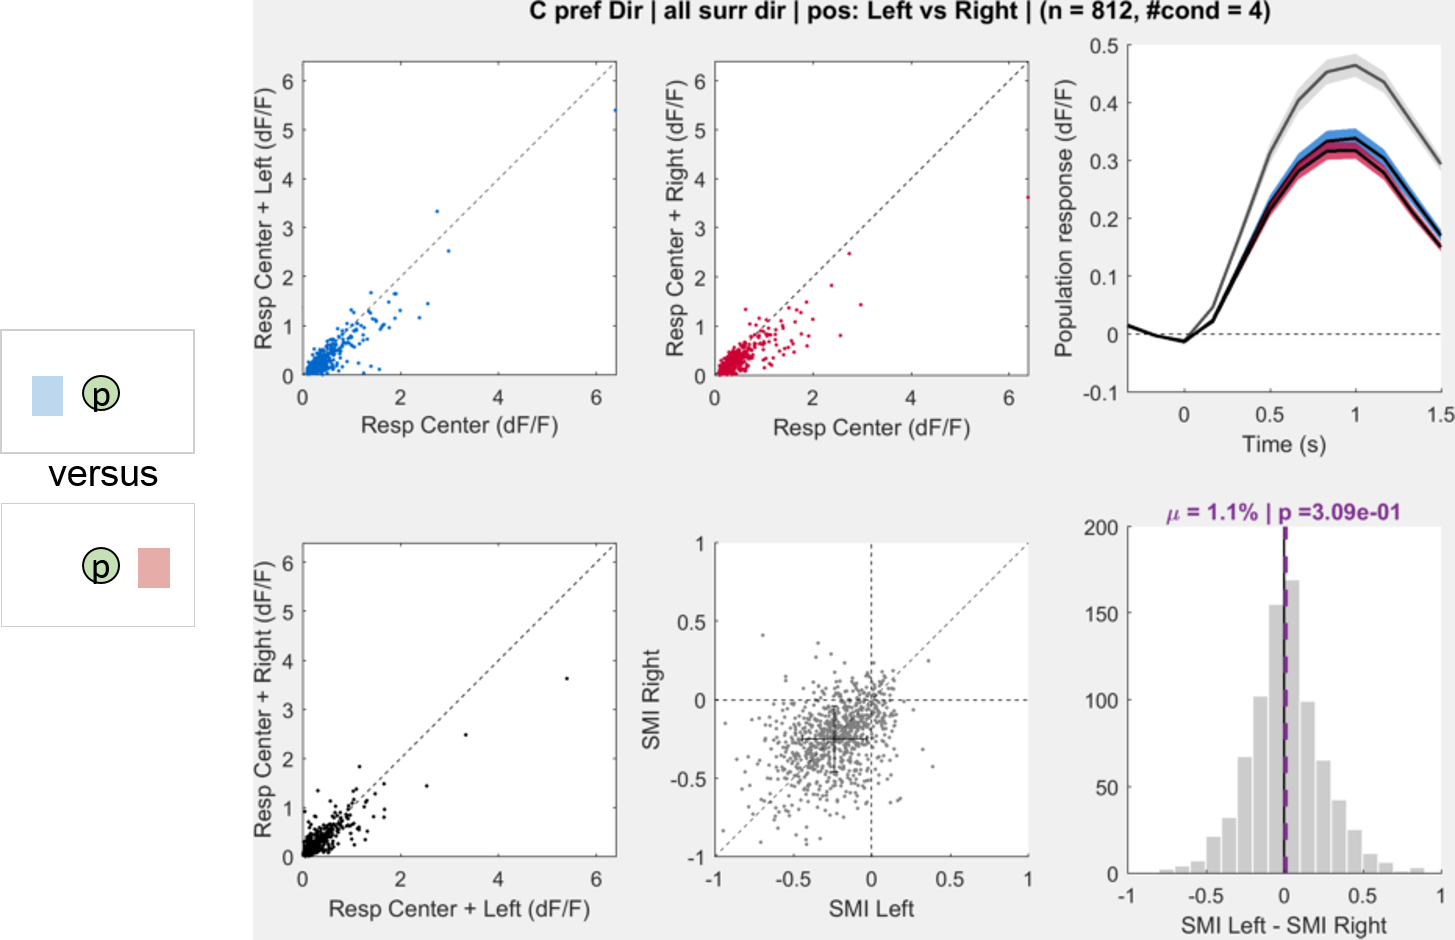
\includegraphics[width=11cm,height=11cm,keepaspectratio]{Figures/7.Results/population/sel/diagrams/2.png} 
%\caption{13_popPlots_VisROIs_CprefDir_Snumber} 
\end{figure}


%\begin{figure}[H] \centering 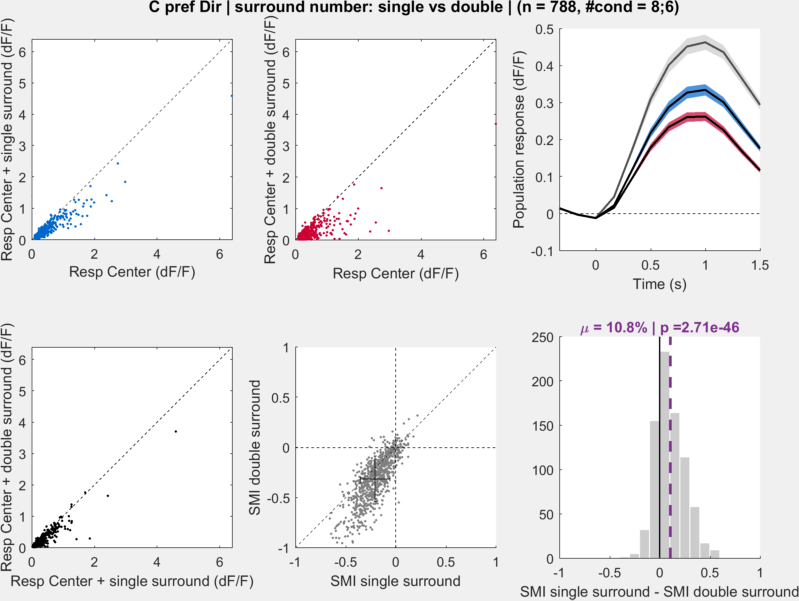
\includegraphics[width=11cm,height=11cm,keepaspectratio]{Figures/7.Results/population/sel/13_popPlots_VisROIs_CprefDir_Snumber.png} 
%%\caption{13_popPlots_VisROIs_CprefDir_Snumber} 
%\end{figure}
%
%\begin{figure}[H] \centering 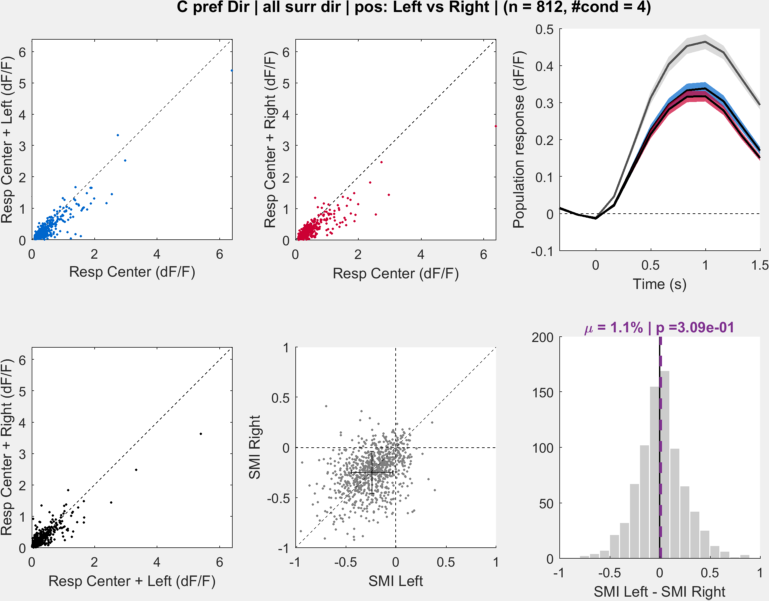
\includegraphics[width=11cm,height=11cm,keepaspectratio]{Figures/7.Results/population/sel/14_popPlots_VisROIs_CprefDir_SposLeftRight.png} 
%%\caption{14_popPlots_VisROIs_CprefDir_SposLeftRight} 
%\end{figure}

\begin{figure}[H] \centering 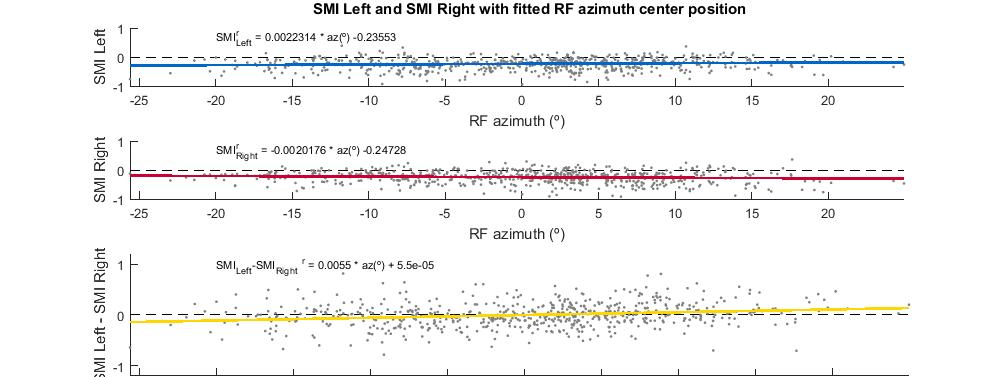
\includegraphics[width=11cm,height=11cm,keepaspectratio]{Figures/7.Results/population/sel/15_LeftversusRightwithAzimuth.jpg} 
%\caption{15_LeftversusRightwithAzimuth} 
\end{figure}

\begin{figure}[H] \centering 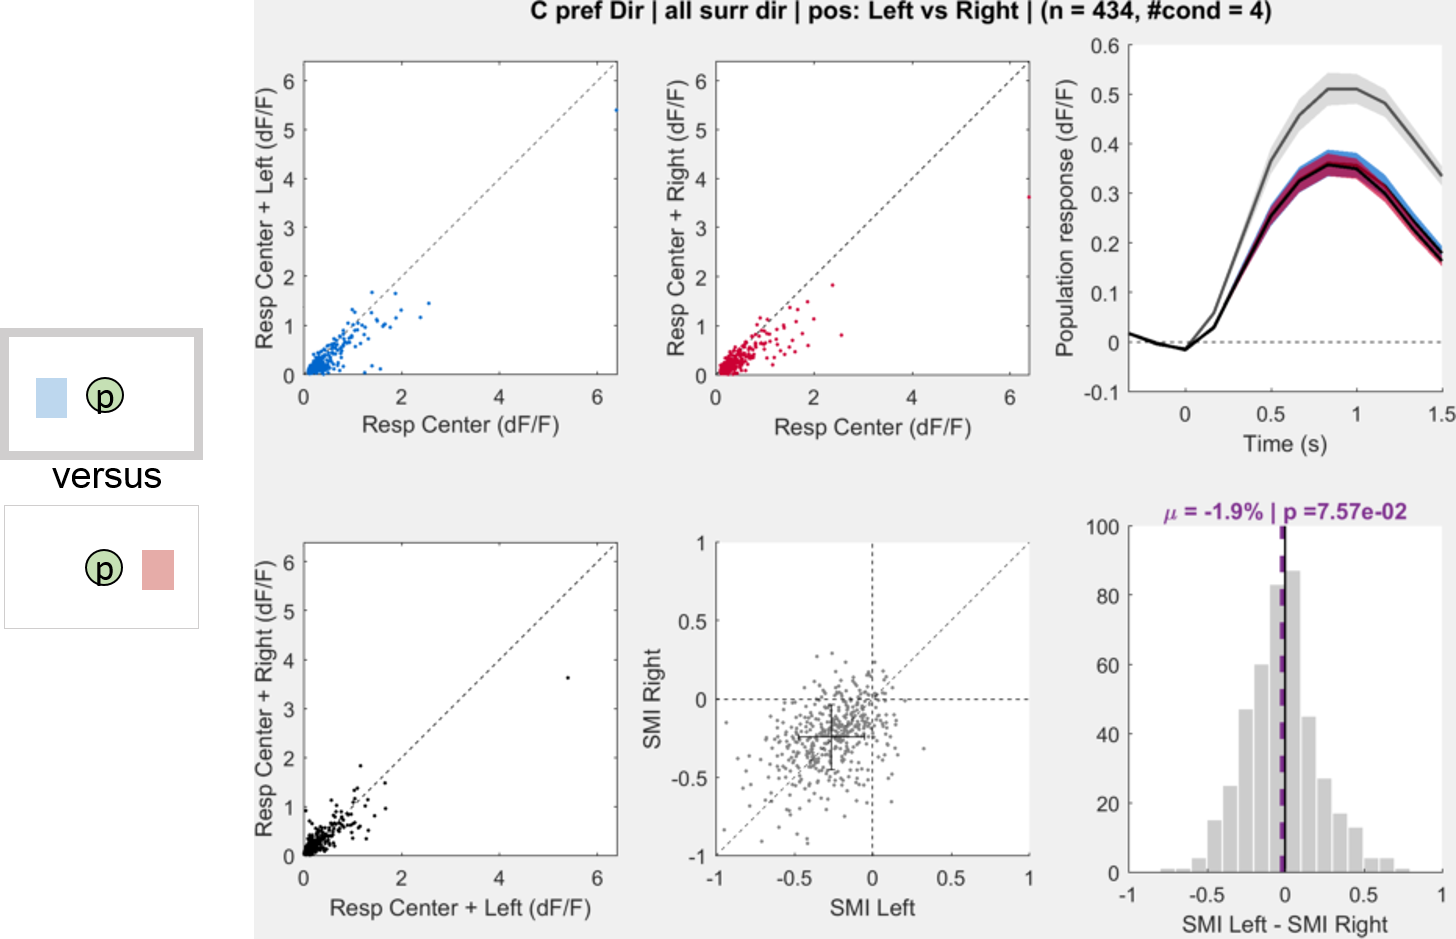
\includegraphics[width=11cm,height=11cm,keepaspectratio]{Figures/7.Results/population/sel/diagrams/3.png} 
%\caption{13_popPlots_VisROIs_CprefDir_Snumber} 
\end{figure}

\subsubsection{Surround direction effect}

\begin{figure}[H] \centering 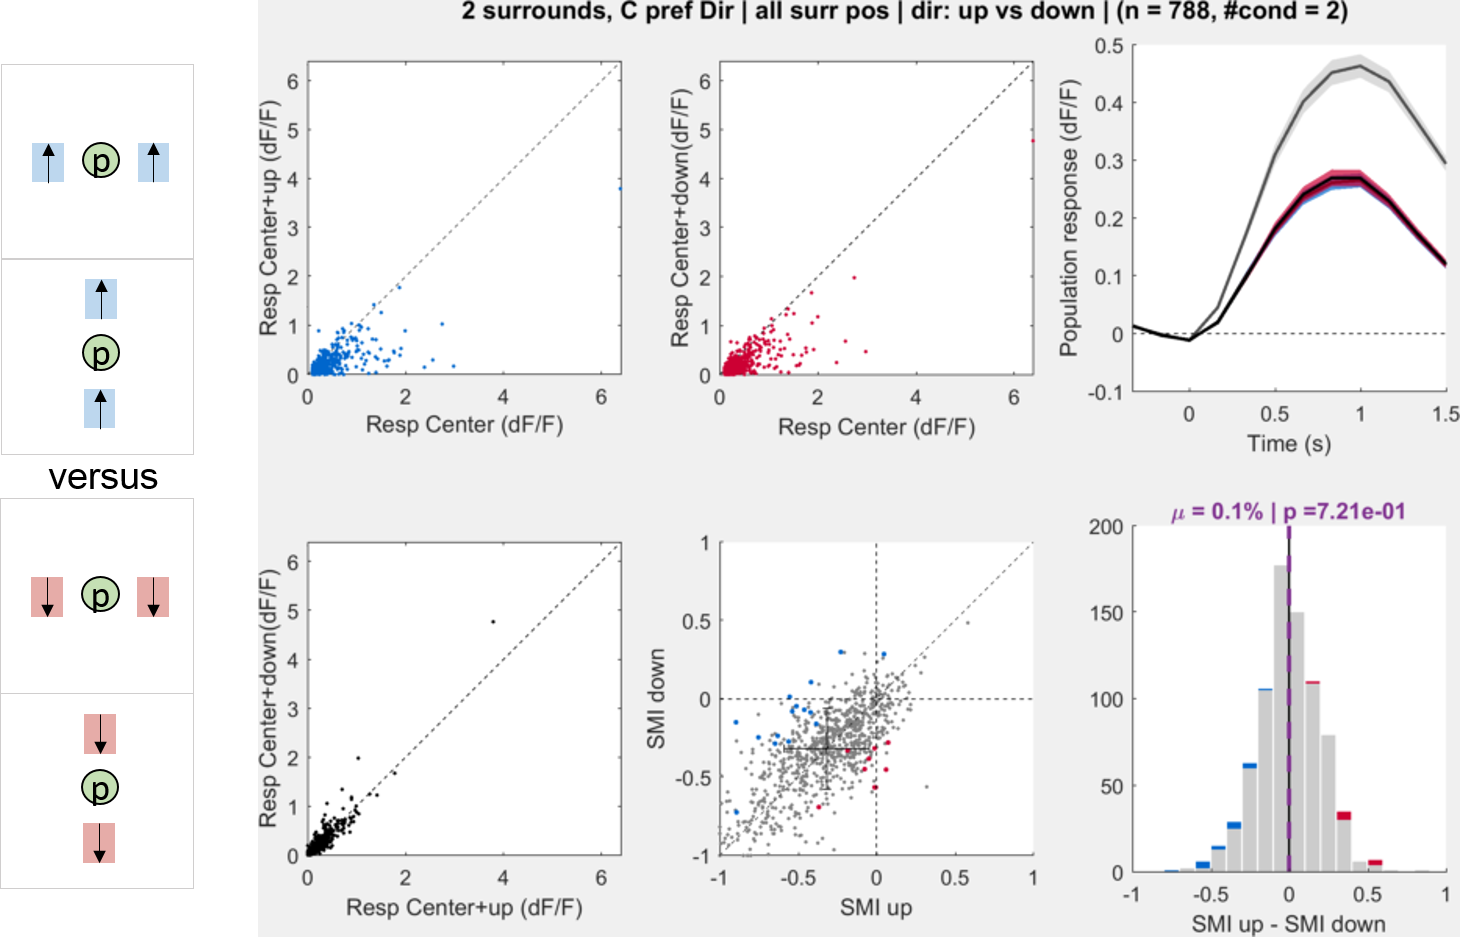
\includegraphics[width=11cm,height=11cm,keepaspectratio]{Figures/7.Results/population/sel/diagrams/4.png} 
%\caption{13_popPlots_VisROIs_CprefDir_Snumber} 
\end{figure}

\begin{figure}[H] \centering 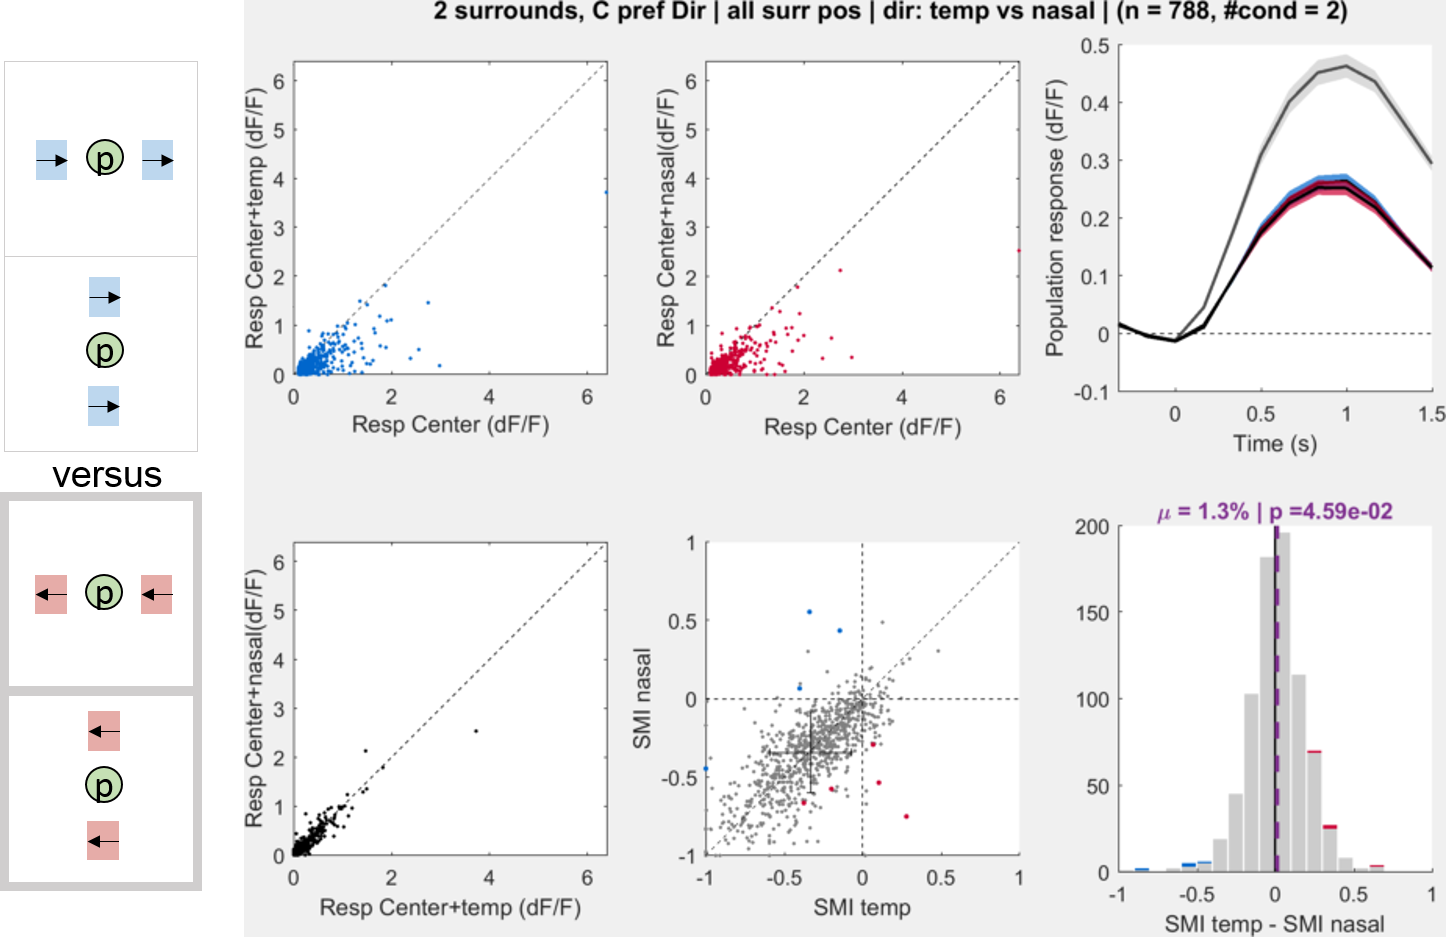
\includegraphics[width=11cm,height=11cm,keepaspectratio]{Figures/7.Results/population/sel/diagrams/5.png} 
%\caption{13_popPlots_VisROIs_CprefDir_Snumber} 
\end{figure}

\subsubsection{Surround orientation effect}

\begin{figure}[H] \centering 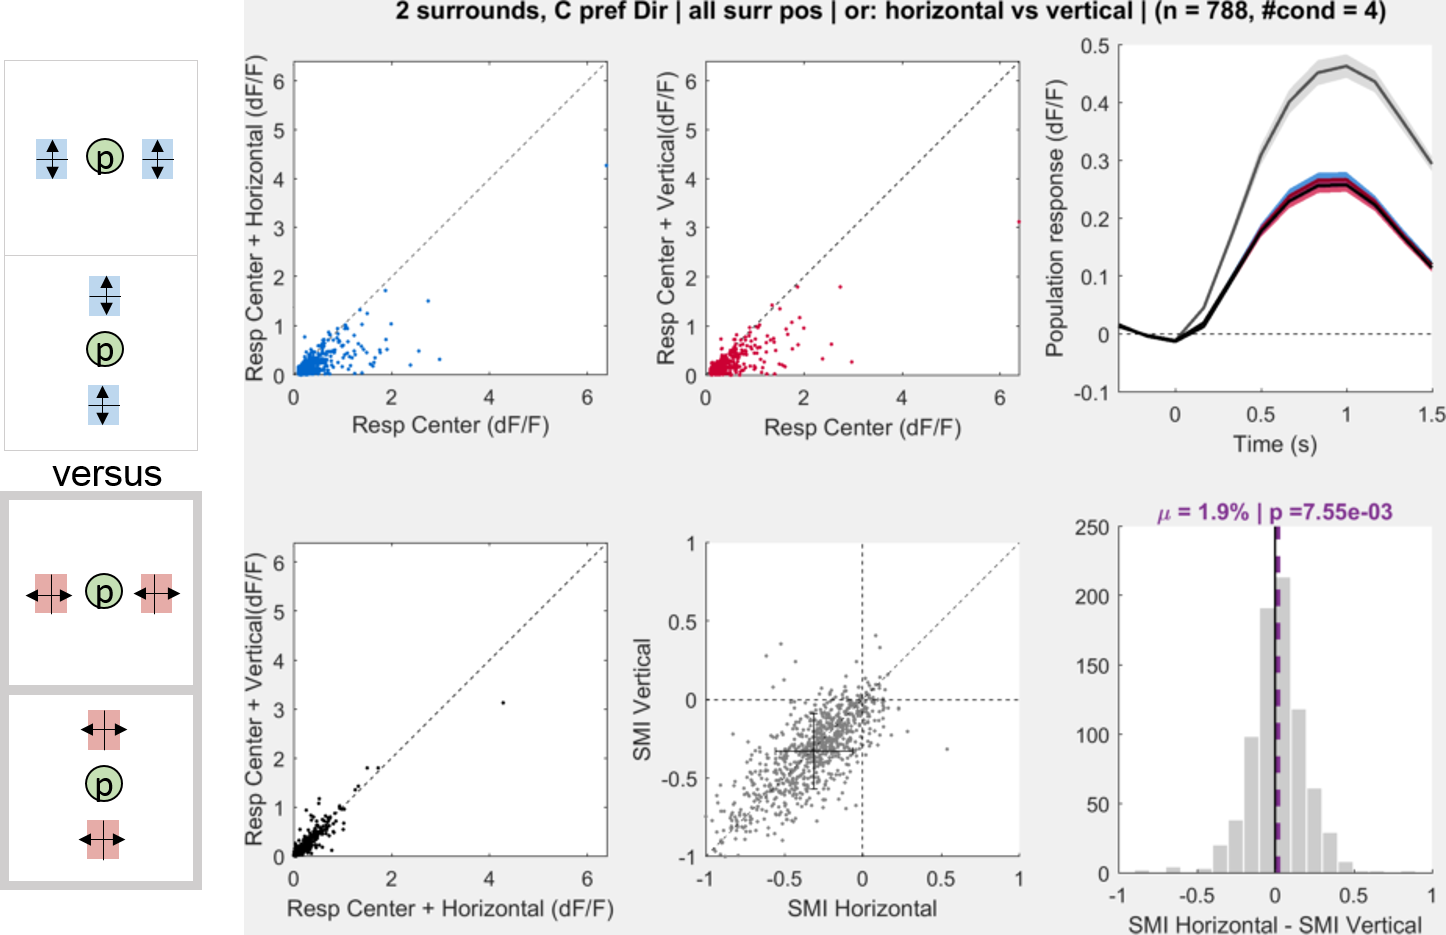
\includegraphics[width=11cm,height=11cm,keepaspectratio]{Figures/7.Results/population/sel/diagrams/6.png} 
%\caption{13_popPlots_VisROIs_CprefDir_Snumber} 
\end{figure}

\subsubsection{Surround orientation alignment effect (position and orientation)}

\begin{figure}[H] \centering 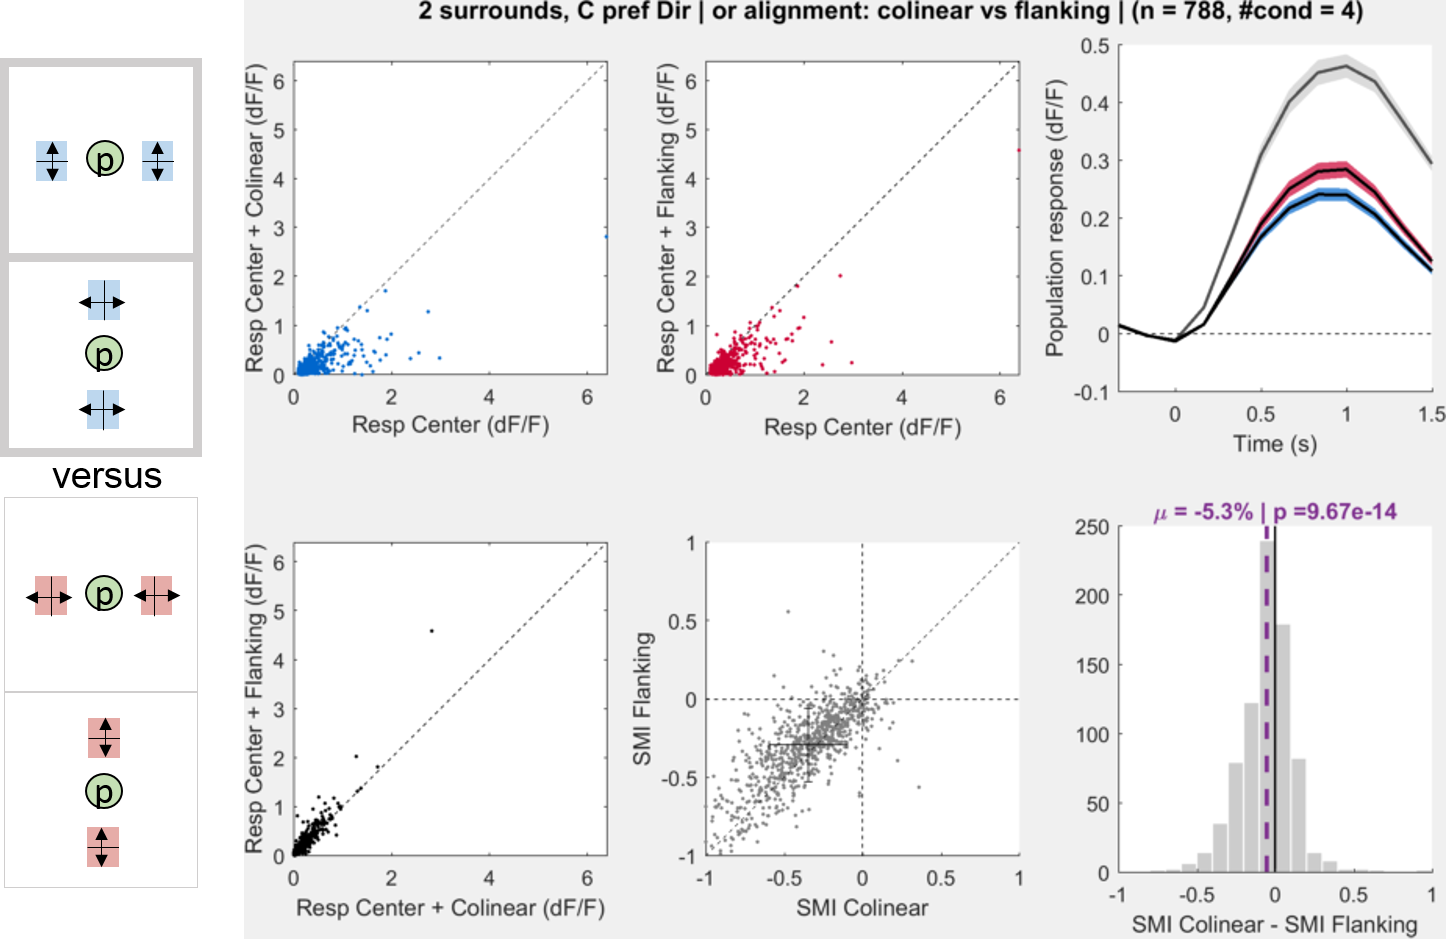
\includegraphics[width=11cm,height=11cm,keepaspectratio]{Figures/7.Results/population/sel/diagrams/7.png} 
%\caption{13_popPlots_VisROIs_CprefDir_Snumber} 
\end{figure}

\subsubsection{Center and surround relative orientation effect, with center OS preference}

\begin{figure}[H] \centering 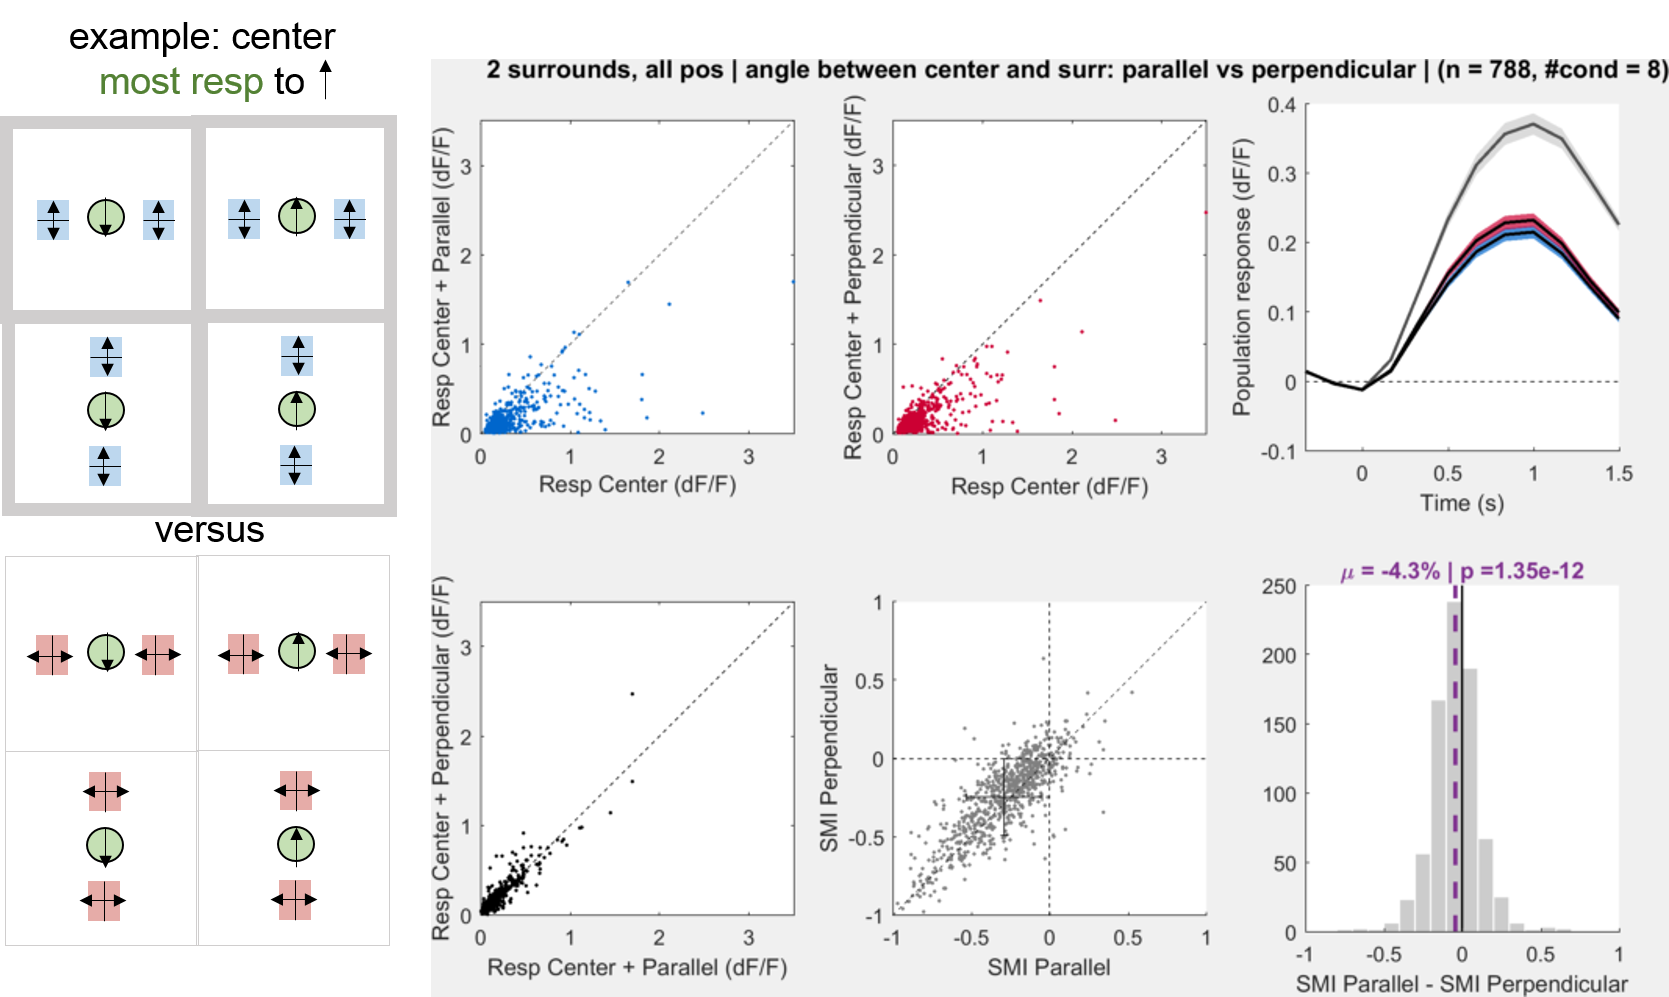
\includegraphics[width=11cm,height=11cm,keepaspectratio]{Figures/7.Results/population/sel/diagrams/8.png} 
%\caption{13_popPlots_VisROIs_CprefDir_Snumber} 
\end{figure}

\begin{figure}[H] \centering 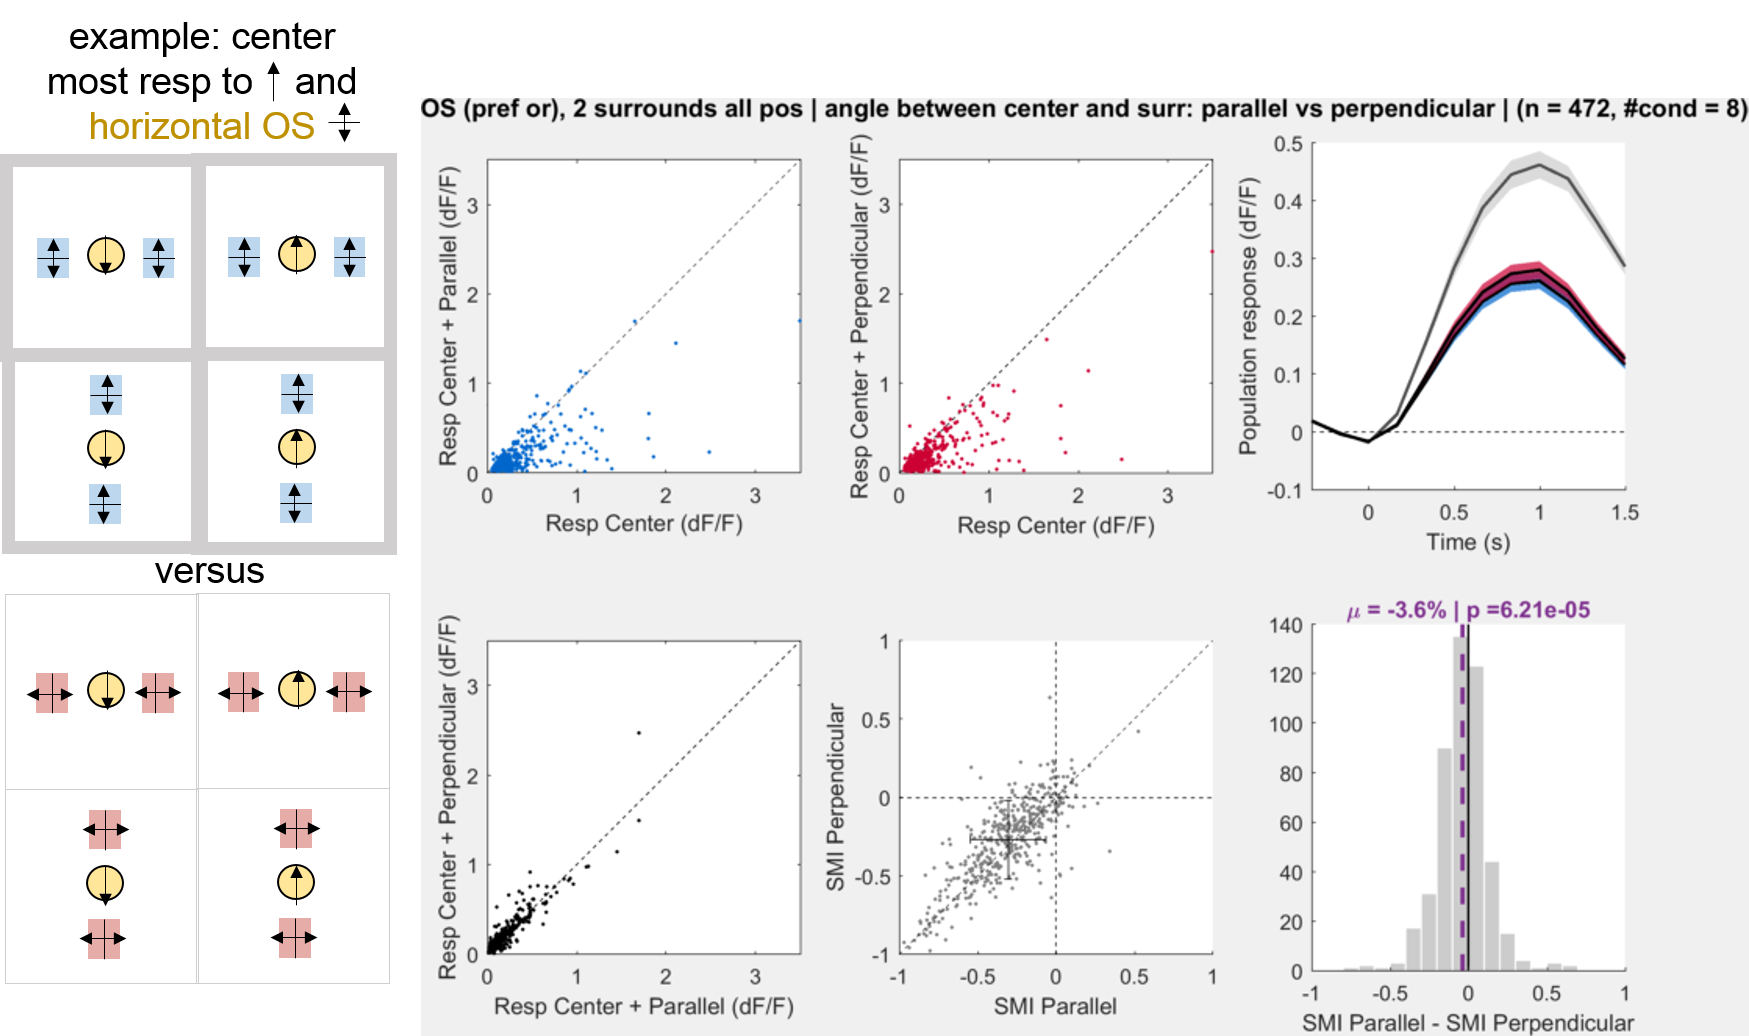
\includegraphics[width=11cm,height=11cm,keepaspectratio]{Figures/7.Results/population/sel/diagrams/9.png} 
%\caption{13_popPlots_VisROIs_CprefDir_Snumber} 
\end{figure}

\begin{figure}[H] \centering 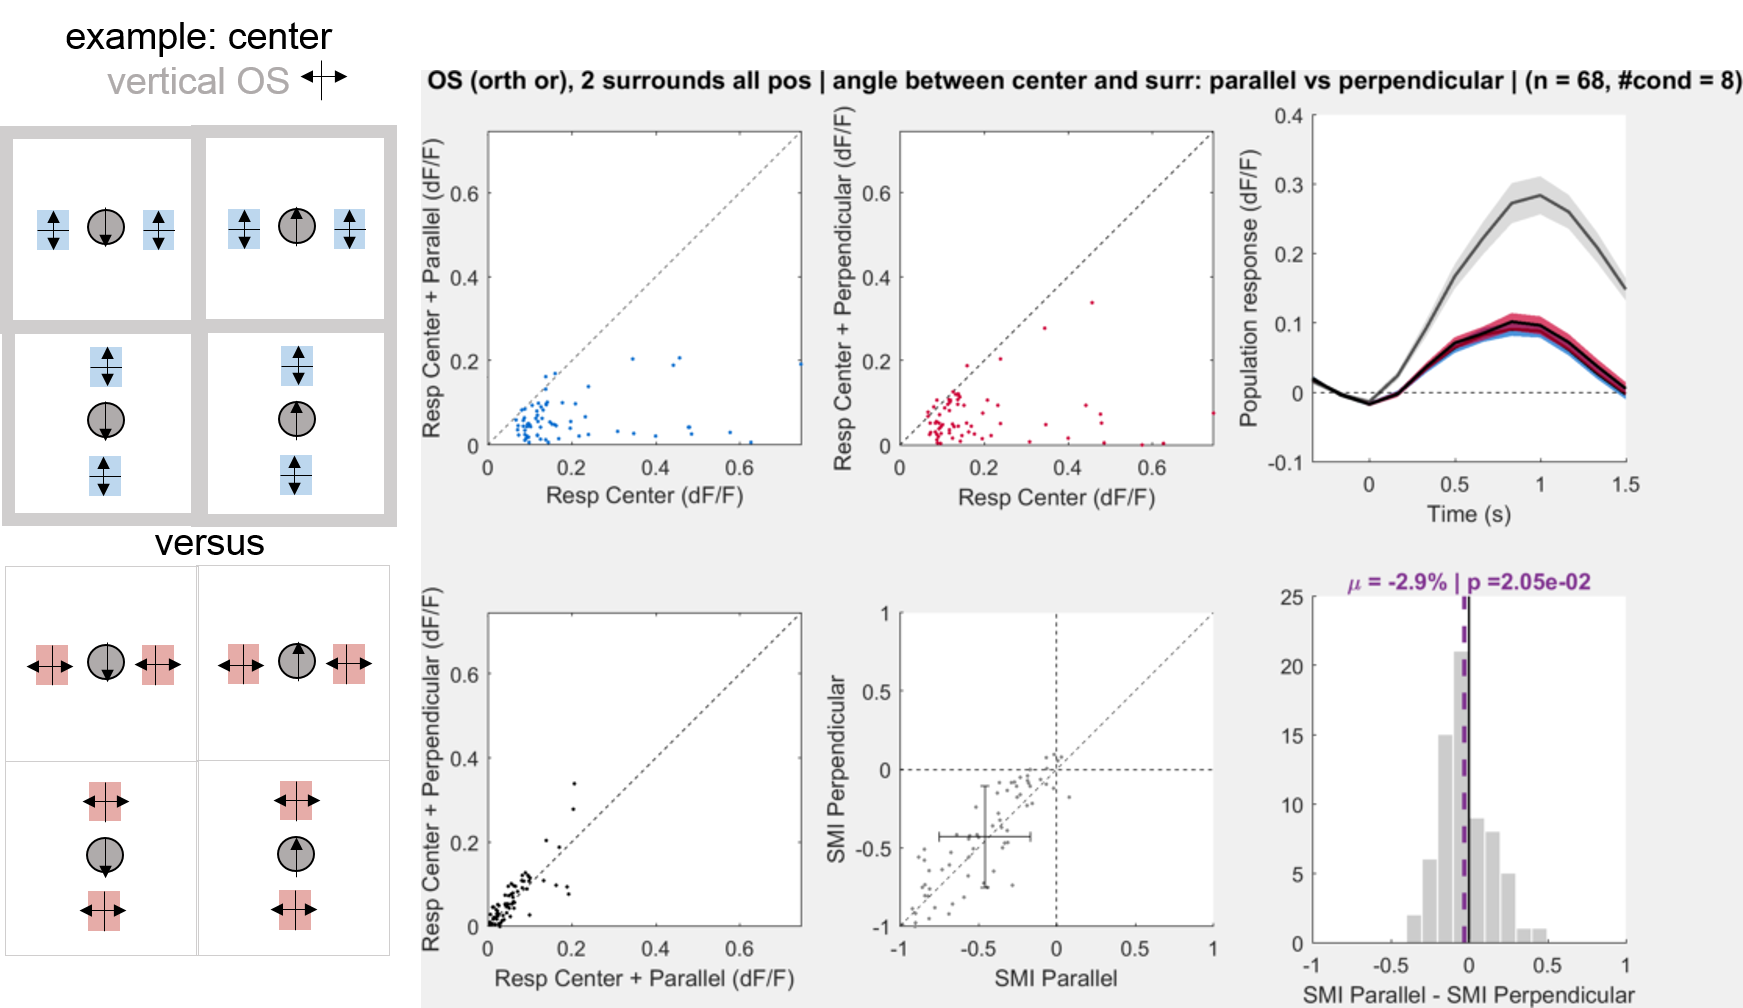
\includegraphics[width=11cm,height=11cm,keepaspectratio]{Figures/7.Results/population/sel/diagrams/10.png} 
%\caption{13_popPlots_VisROIs_CprefDir_Snumber} 
\end{figure}

\subsubsection{Interactions between surround orientation alignment and surround-center relative orientation effects}

\begin{figure}[H] \centering 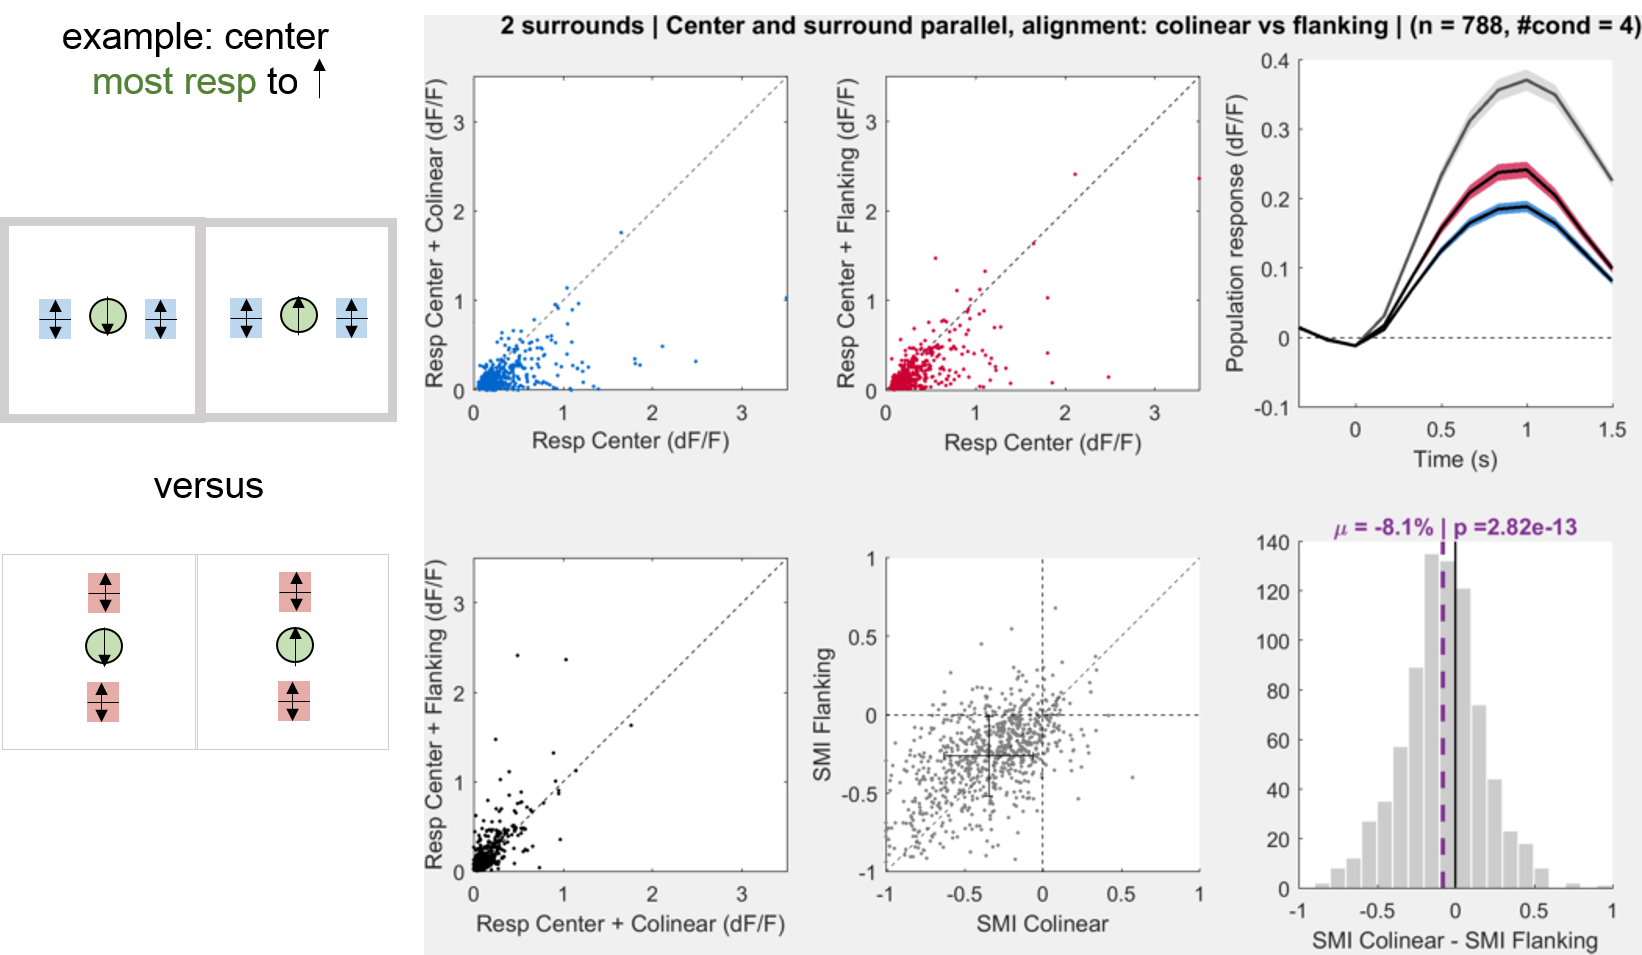
\includegraphics[width=11cm,height=11cm,keepaspectratio]{Figures/7.Results/population/sel/diagrams/11.png} 
%\caption{13_popPlots_VisROIs_CprefDir_Snumber} 
\end{figure}

\begin{figure}[H] \centering 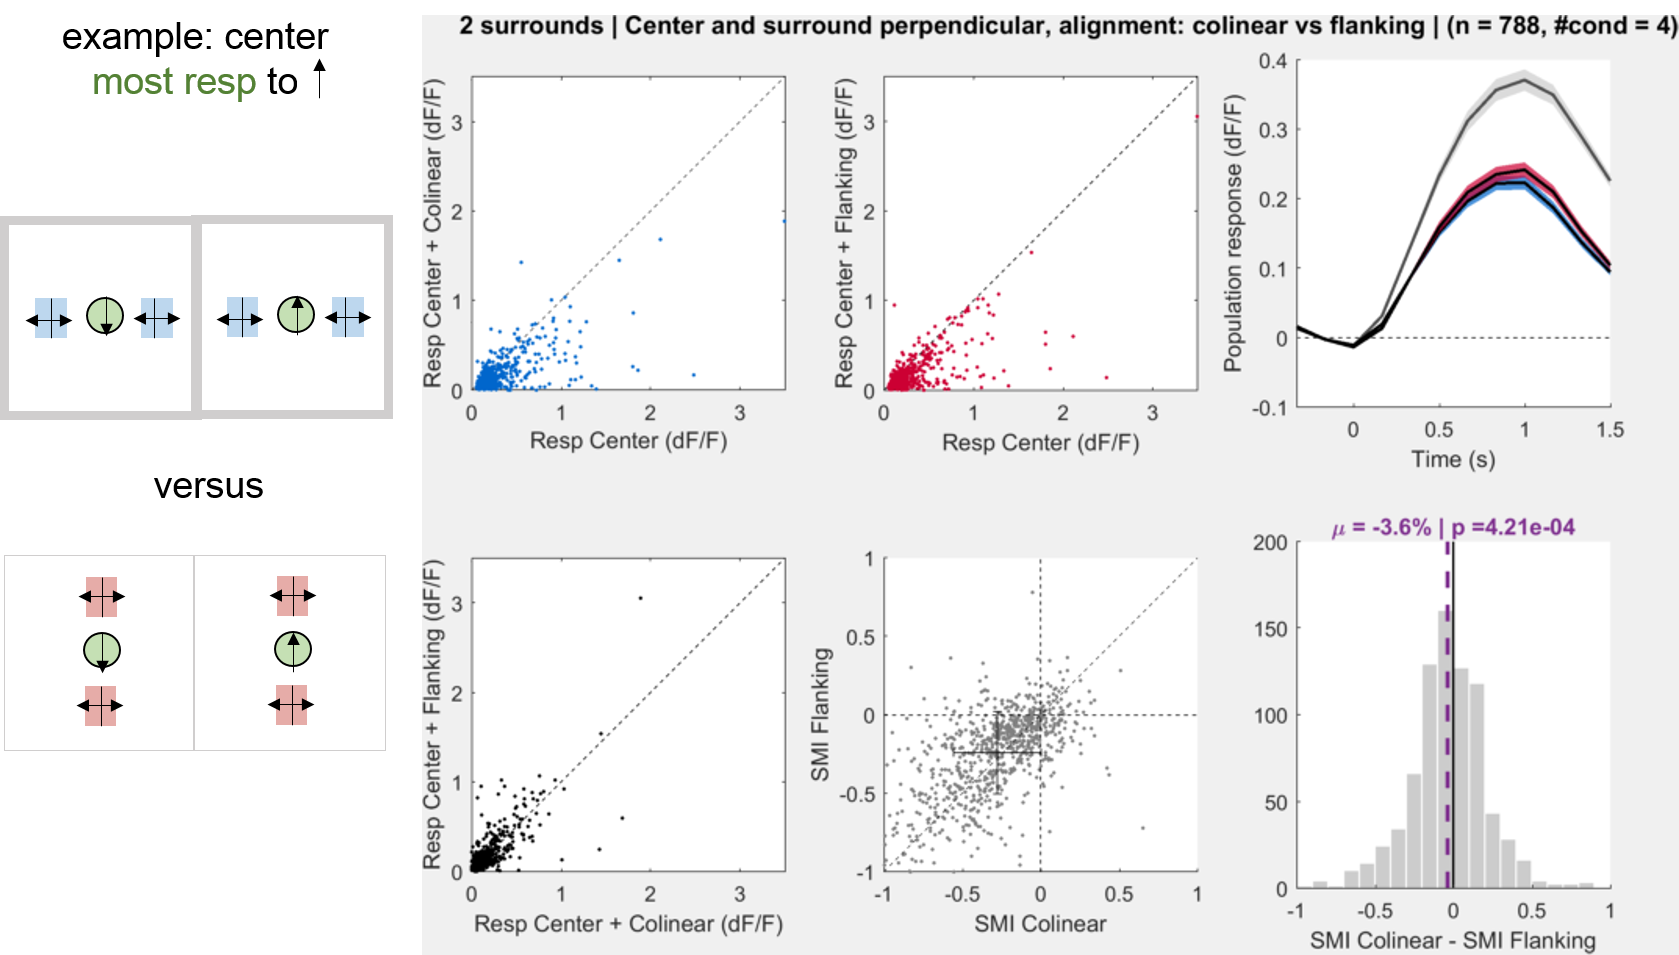
\includegraphics[width=11cm,height=11cm,keepaspectratio]{Figures/7.Results/population/sel/diagrams/12.png} 
%\caption{13_popPlots_VisROIs_CprefDir_Snumber} 
\end{figure}

\begin{figure}[H] \centering 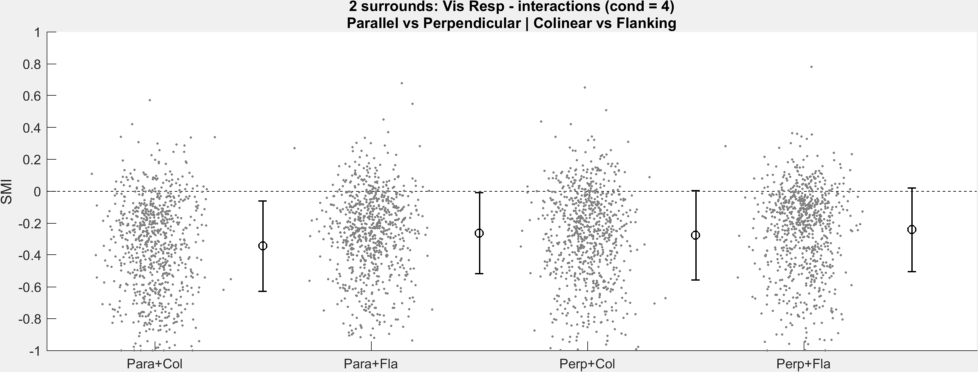
\includegraphics[width=11cm,height=11cm,keepaspectratio]{Figures/7.Results/population/sel/26_popPlots_VisROIs_Cor_2SalignmentAngle.png} 
%\caption{26_popPlots_VisROIs_Cor_2SalignmentAngle} 
\end{figure}

\subsubsection{Interactions between surround orientation alignment, surround-center relative orientation effects and center OS preference}

\begin{figure}[H] \centering 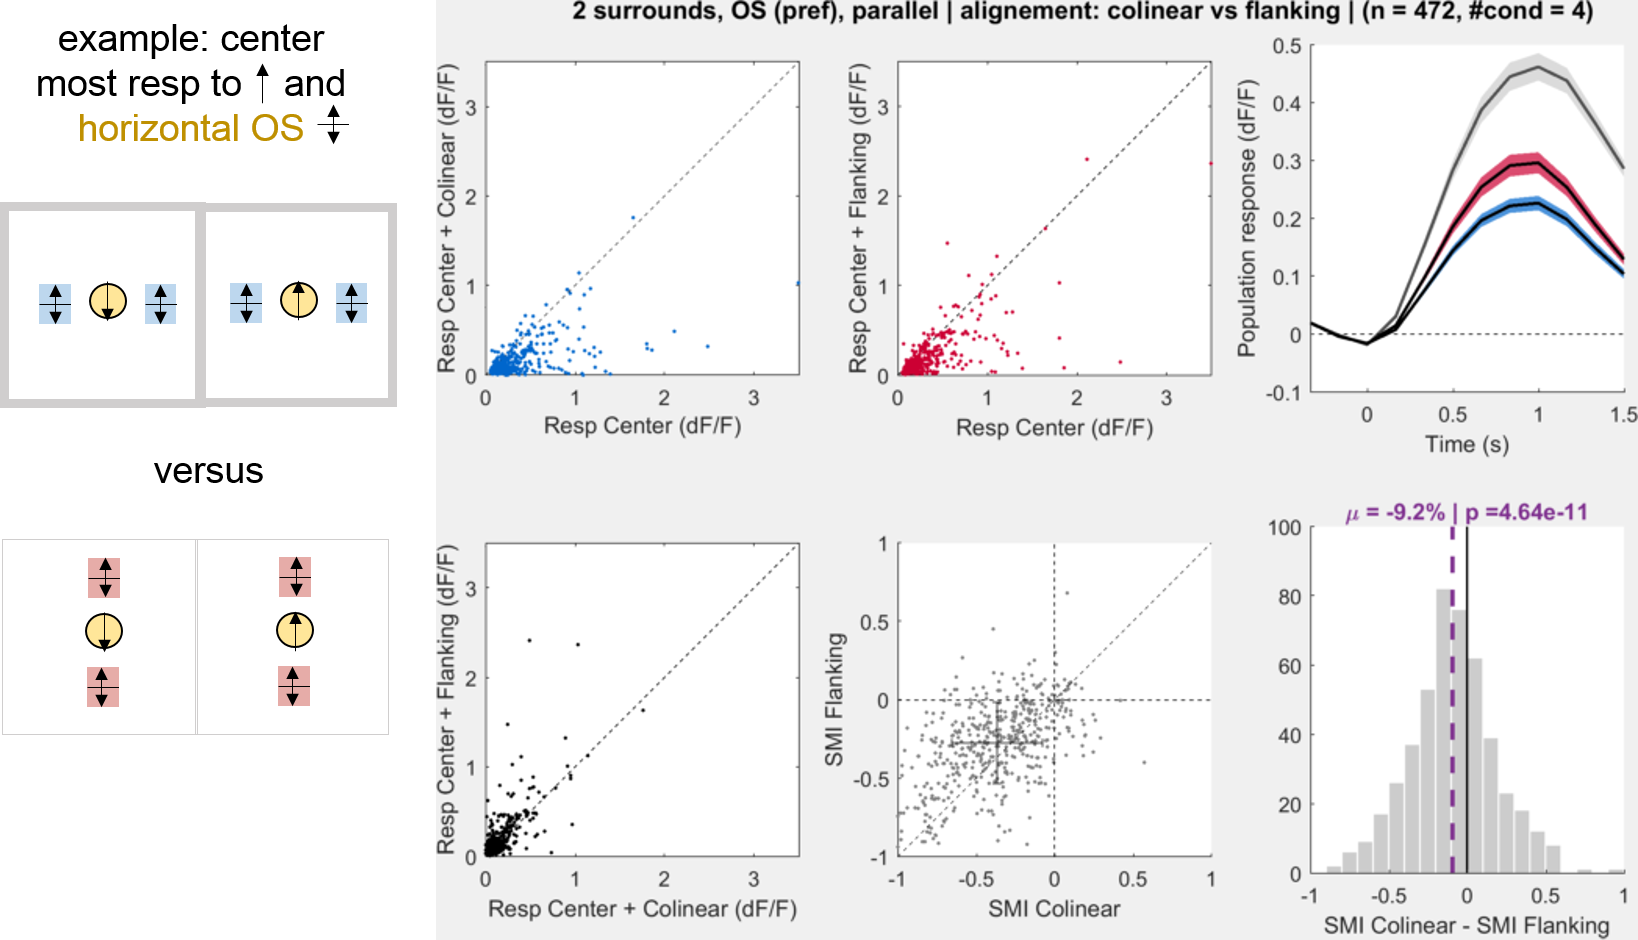
\includegraphics[width=11cm,height=11cm,keepaspectratio]{Figures/7.Results/population/sel/diagrams/13.png} 
%\caption{13_popPlots_VisROIs_CprefDir_Snumber} 
\end{figure}

\begin{figure}[H] \centering 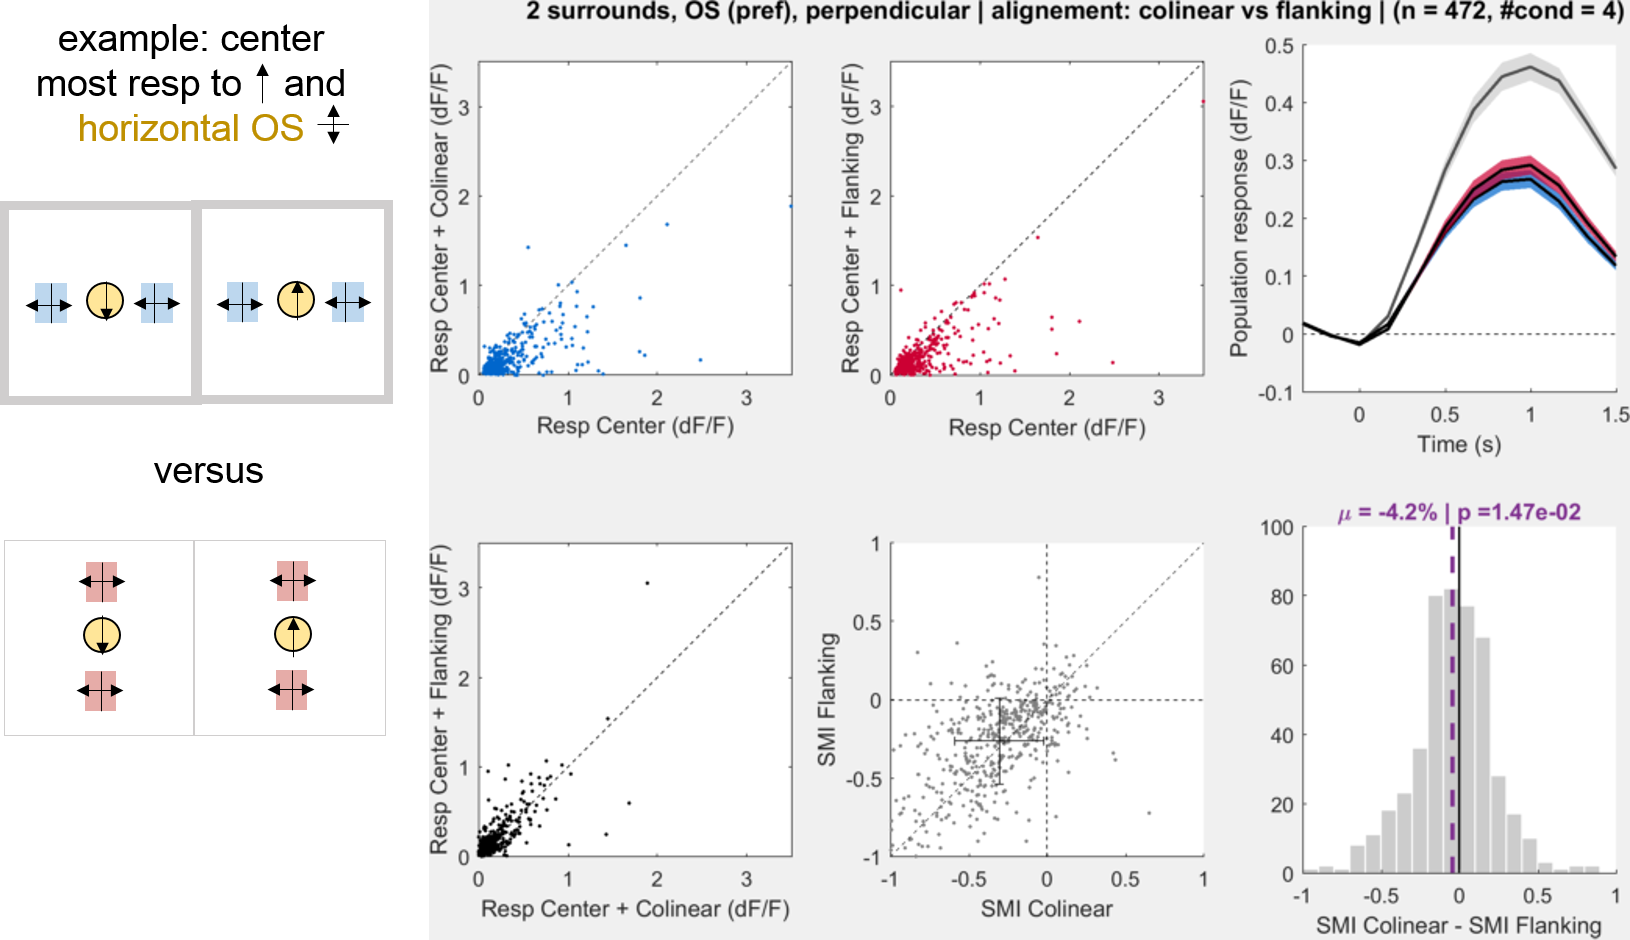
\includegraphics[width=11cm,height=11cm,keepaspectratio]{Figures/7.Results/population/sel/diagrams/14.png} 
%\caption{13_popPlots_VisROIs_CprefDir_Snumber} 
\end{figure}

\begin{figure}[H] \centering 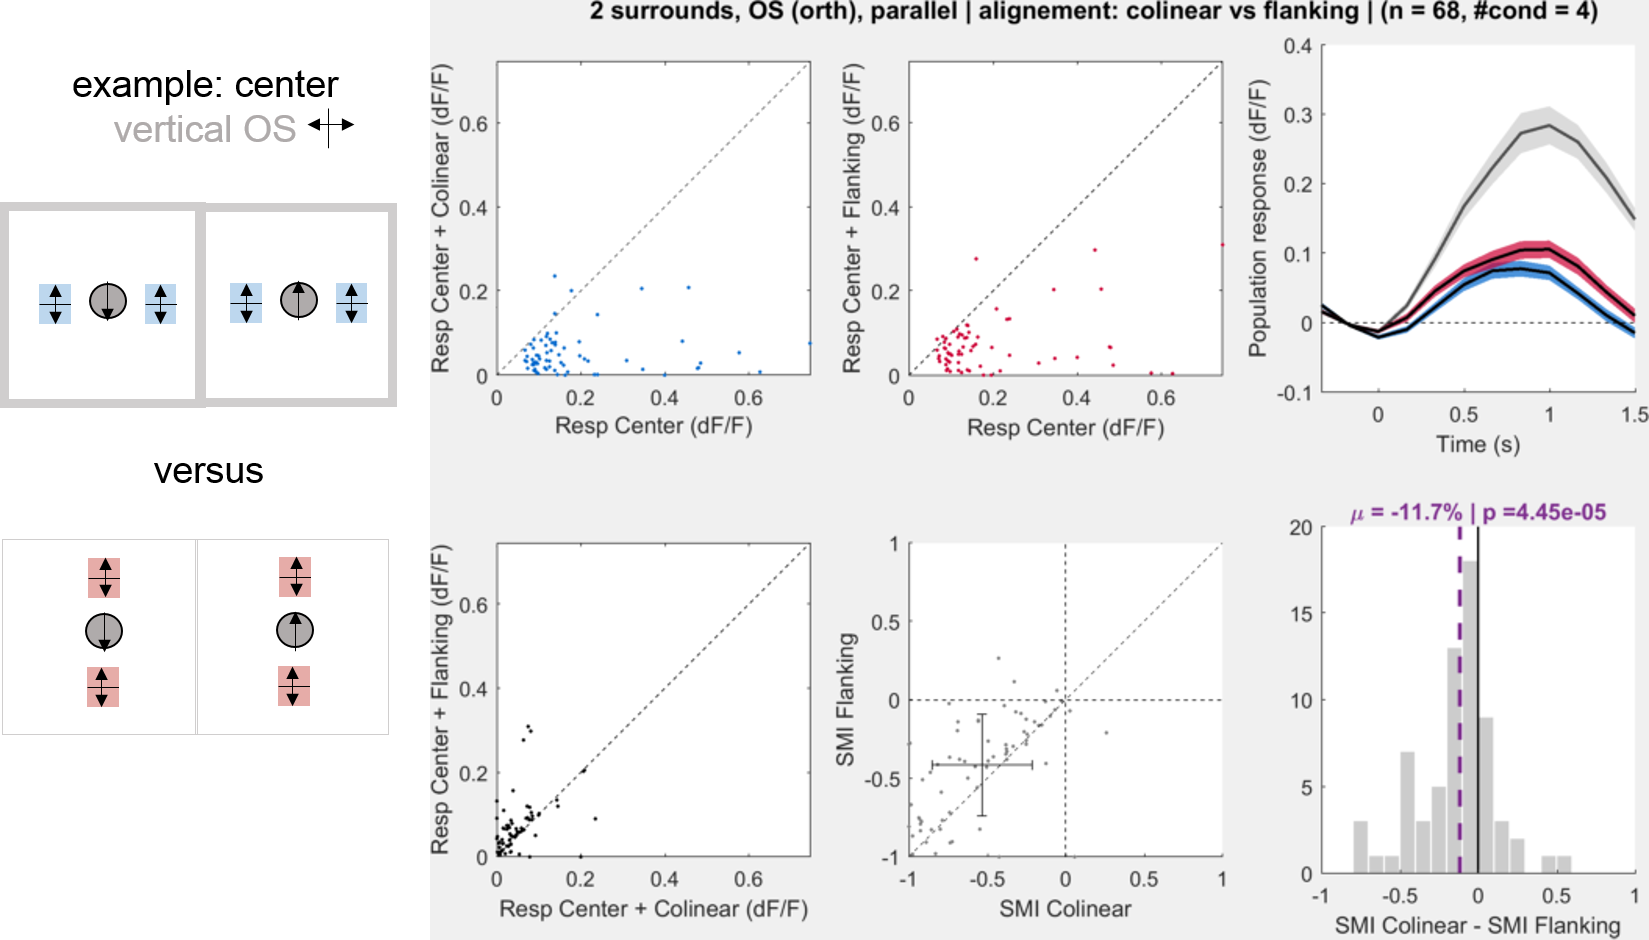
\includegraphics[width=11cm,height=11cm,keepaspectratio]{Figures/7.Results/population/sel/diagrams/15.png} 
%\caption{13_popPlots_VisROIs_CprefDir_Snumber} 
\end{figure}

\begin{figure}[H] \centering 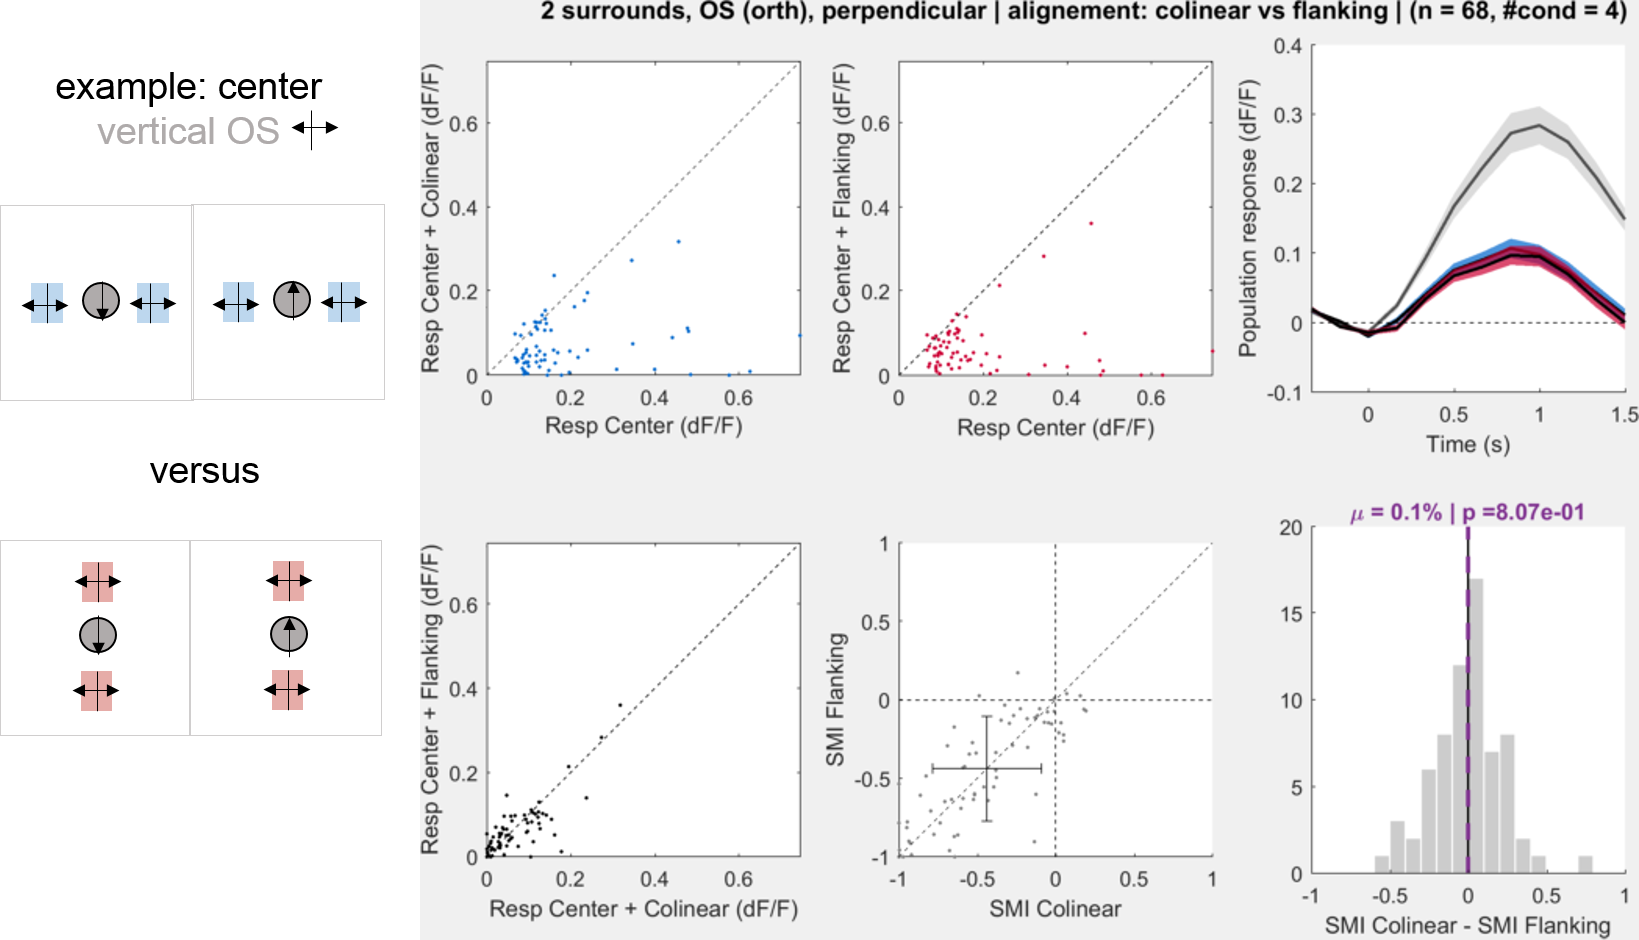
\includegraphics[width=11cm,height=11cm,keepaspectratio]{Figures/7.Results/population/sel/diagrams/16.png} 
%\caption{13_popPlots_VisROIs_CprefDir_Snumber} 
\end{figure}

\begin{figure}[H] \centering 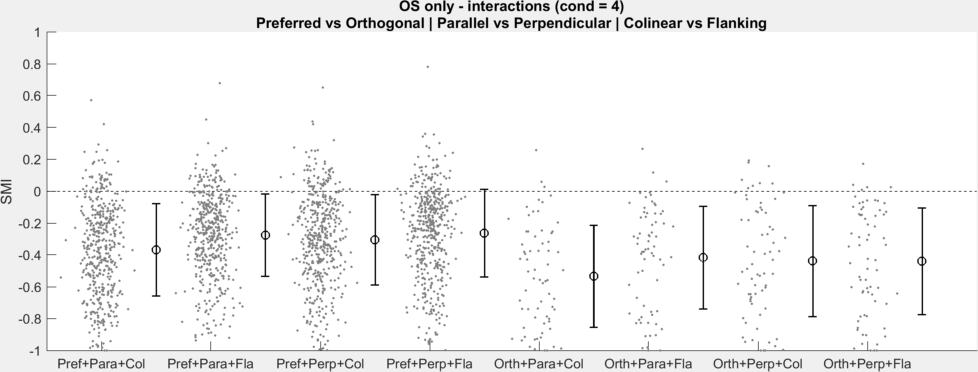
\includegraphics[width=11cm,height=11cm,keepaspectratio]{Figures/7.Results/population/sel/31_popPlots_VisROIs_COS_2SalignmentAngle.png} 
%\caption{31_popPlots_VisROIs_COS_2SalignmentAngle} 
\end{figure}

\subsubsection{Surround direction alignment effect (direction and position)}

\begin{figure}[H] \centering 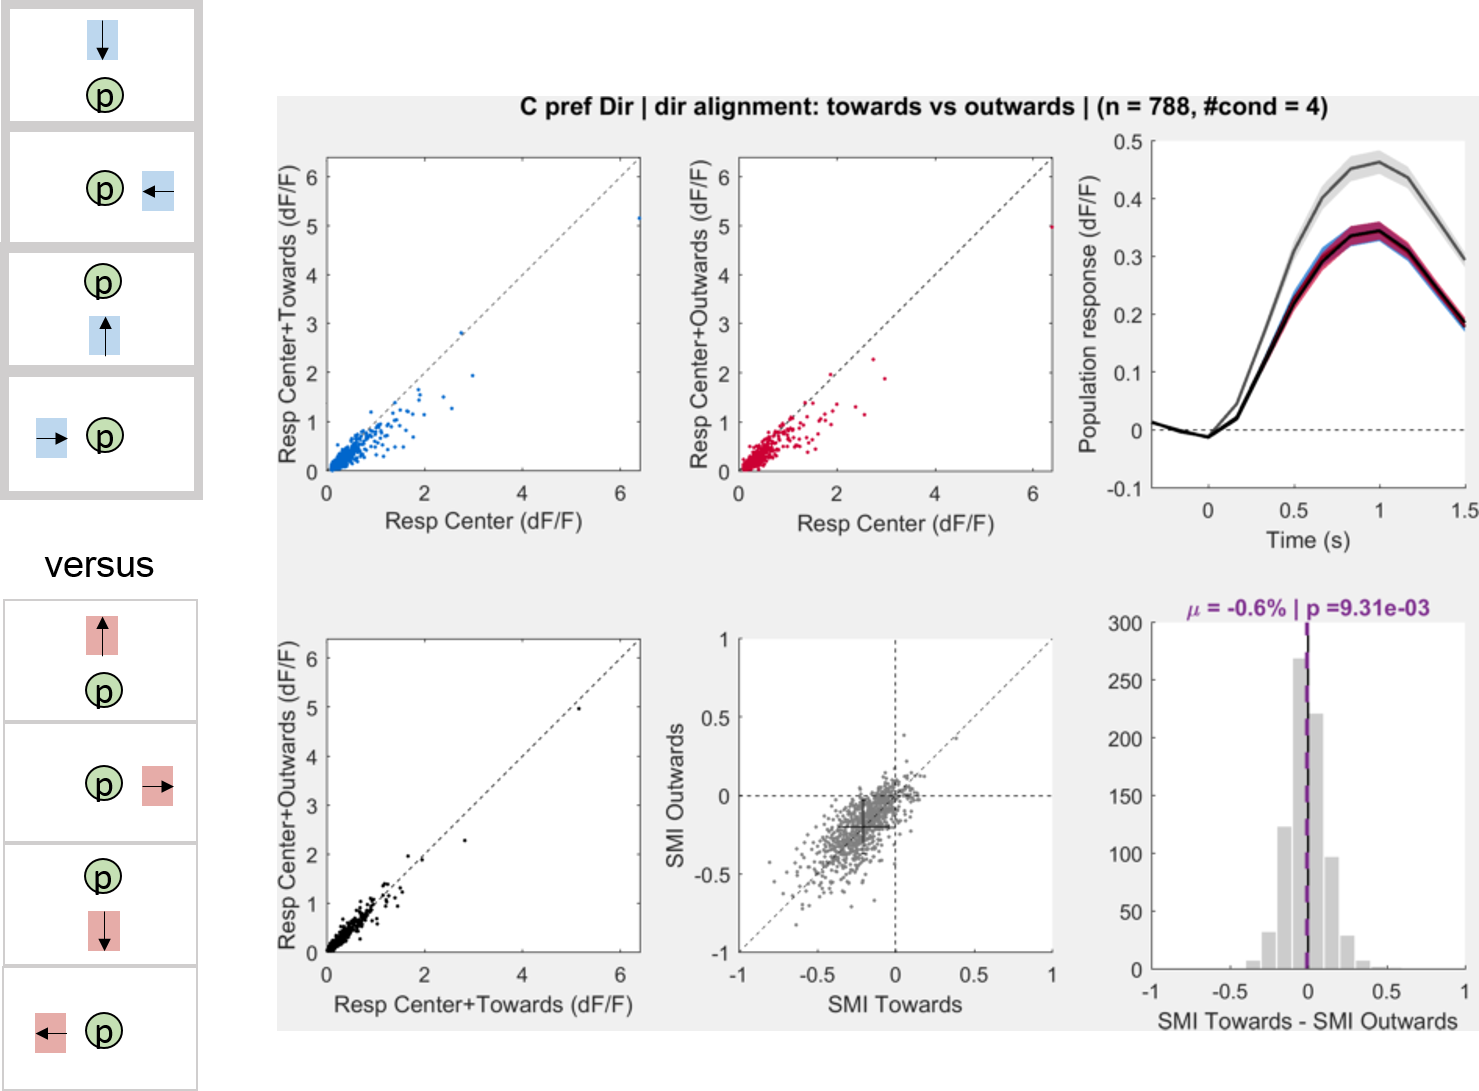
\includegraphics[width=11cm,height=11cm,keepaspectratio]{Figures/7.Results/population/sel/diagrams/17.png} 
%\caption{13_popPlots_VisROIs_CprefDir_Snumber} 
\end{figure}

\subsubsection{Surround and center relative direction effect}

\begin{figure}[H] \centering 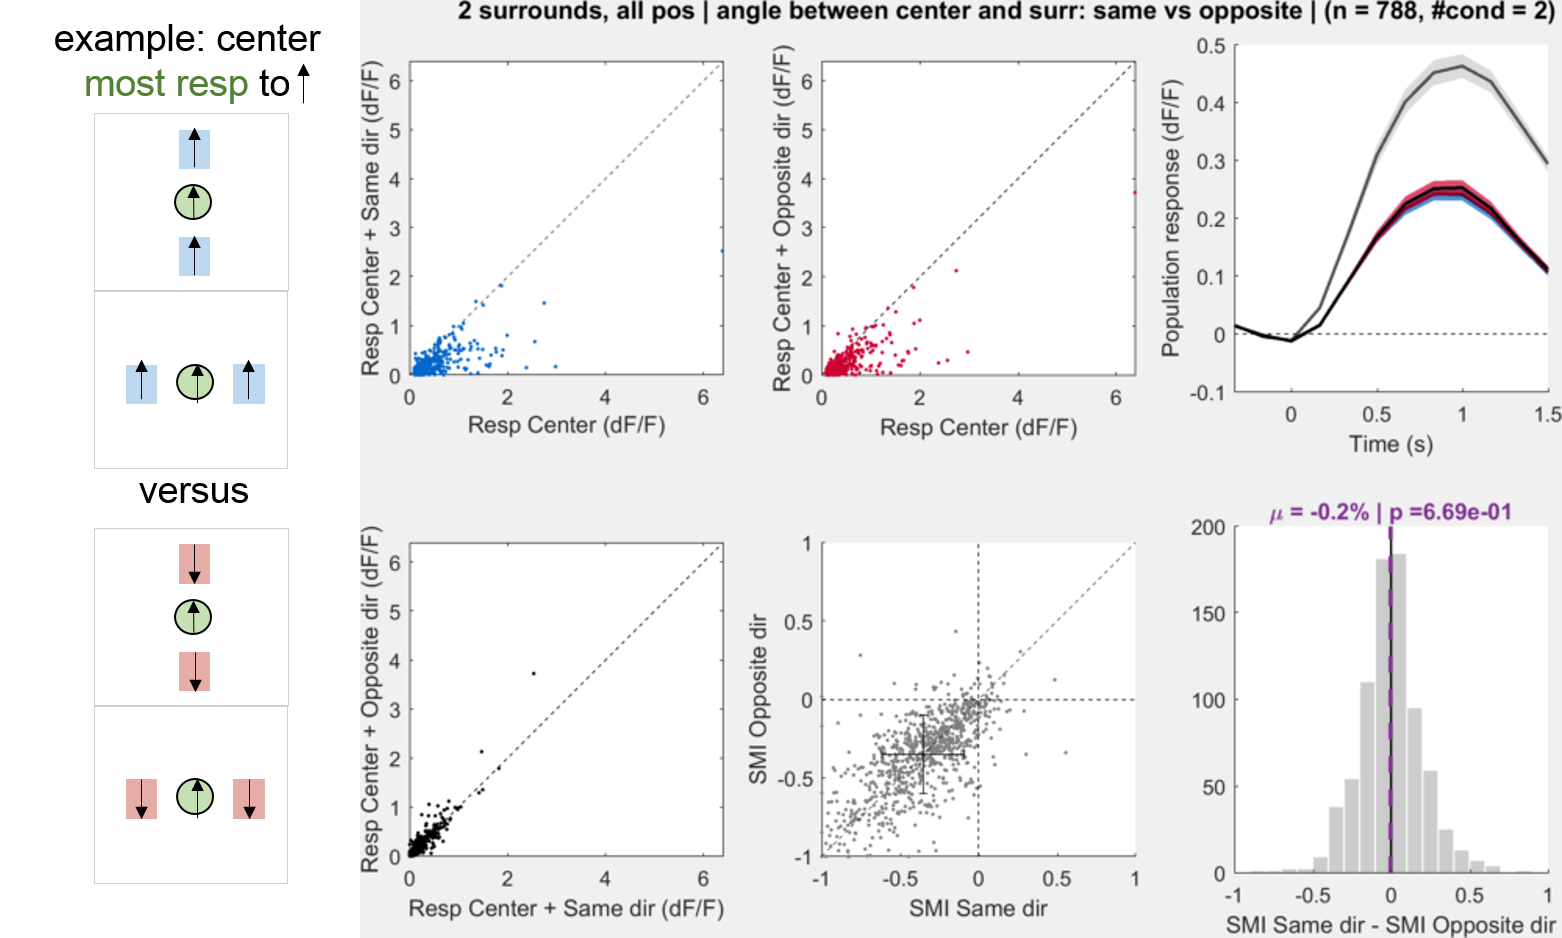
\includegraphics[width=11cm,height=11cm,keepaspectratio]{Figures/7.Results/population/sel/diagrams/18.png} 
%\caption{13_popPlots_VisROIs_CprefDir_Snumber} 
\end{figure}

\subsubsection{Interactions between direction alignment, surround-center relative direction effects and center DS preference}

\begin{figure}[H] \centering \includegraphics[width=11cm,height=11cm,keepaspectratio]{Figures/7.Results/population/sel/diagrams/19.png} 
%\caption{13_popPlots_VisROIs_CprefDir_Snumber} 
\end{figure}

\begin{figure}[H] \centering \includegraphics[width=11cm,height=11cm,keepaspectratio]{Figures/7.Results/population/sel/diagrams/20.png} 
%\caption{13_popPlots_VisROIs_CprefDir_Snumber} 
\end{figure}

\begin{figure}[H] \centering \includegraphics[width=11cm,height=11cm,keepaspectratio]{Figures/7.Results/population/sel/diagrams/21.png} 
%\caption{13_popPlots_VisROIs_CprefDir_Snumber} 
\end{figure}

%outros
%
%\begin{figure}[H] \centering \includegraphics[width=11cm,height=11cm,keepaspectratio]{Figures/7.Results/population/sel/16_popPlots_VisROIs_CprefDir_SposLeftRight_rfCenter.png} 
%%\caption{16_popPlots_VisROIs_CprefDir_SposLeftRight_rfCenter} 
%\end{figure}
%
%\begin{figure}[H] \centering \includegraphics[width=11cm,height=11cm,keepaspectratio]{Figures/7.Results/population/sel/17_popPlots_VisROIs_CprefDir_2SdirUpDown.png} 
%%\caption{17_popPlots_VisROIs_CprefDir_2SdirUpDown} 
%\end{figure}
%
%\begin{figure}[H] \centering \includegraphics[width=11cm,height=11cm,keepaspectratio]{Figures/7.Results/population/sel/18_popPlots_VisROIs_CprefDir_2SdirTemporalNasal.png} 
%%\caption{18_popPlots_VisROIs_CprefDir_2SdirTemporalNasal} 
%\end{figure}
%
%\begin{figure}[H] \centering \includegraphics[width=11cm,height=11cm,keepaspectratio]{Figures/7.Results/population/sel/19_popPlots_VisROIs_CprefDir_2SorHorizontalVertical.png} 
%%\caption{19_popPlots_VisROIs_CprefDir_2SorHorizontalVertical} 
%\end{figure}
%
%\begin{figure}[H] \centering \includegraphics[width=11cm,height=11cm,keepaspectratio]{Figures/7.Results/population/sel/20_popPlots_VisROIs_CprefDir_2SalignmentColinearFlanking.png} 
%%\caption{20_popPlots_VisROIs_CprefDir_2SalignmentColinearFlanking} 
%\end{figure}
%
%\begin{figure}[H] \centering \includegraphics[width=11cm,height=11cm,keepaspectratio]{Figures/7.Results/population/sel/21_popPlots_VisROIs_Cor_2SangleParallelPerpendicular.png} 
%%\caption{21_popPlots_VisROIs_Cor_2SangleParallelPerpendicular} 
%\end{figure}
%
%\begin{figure}[H] \centering \includegraphics[width=11cm,height=11cm,keepaspectratio]{Figures/7.Results/population/sel/22_popPlots_VisROIs_COSprefOr_2SangleParallelPerpendicular.png} 
%%\caption{22_popPlots_VisROIs_COSprefOr_2SangleParallelPerpendicular} 
%\end{figure}
%
%\begin{figure}[H] \centering \includegraphics[width=11cm,height=11cm,keepaspectratio]{Figures/7.Results/population/sel/23_popPlots_VisROIs_COSorthOr_2SangleParallelPerpendicular.png} 
%%\caption{23_popPlots_VisROIs_COSorthOr_2SangleParallelPerpendicular} 
%\end{figure}
%
%\begin{figure}[H] \centering \includegraphics[width=11cm,height=11cm,keepaspectratio]{Figures/7.Results/population/sel/24_popPlots_VisROIs_Cor_2SalignmentColinearFlanking.png} 
%%\caption{24_popPlots_VisROIs_Cor_2SalignmentColinearFlanking} 
%\end{figure}
%
%\begin{figure}[H] \centering \includegraphics[width=11cm,height=11cm,keepaspectratio]{Figures/7.Results/population/sel/25_popPlots_VisROIs_Cor_2SalignmentColinearFlanking2.png} 
%%\caption{25_popPlots_VisROIs_Cor_2SalignmentColinearFlanking2} 
%\end{figure}
%
%\begin{figure}[H] \centering \includegraphics[width=11cm,height=11cm,keepaspectratio]{Figures/7.Results/population/sel/26_popPlots_VisROIs_Cor_2SalignmentAngle.png} 
%%\caption{26_popPlots_VisROIs_Cor_2SalignmentAngle} 
%\end{figure}
%
%\begin{figure}[H] \centering \includegraphics[width=11cm,height=11cm,keepaspectratio]{Figures/7.Results/population/sel/27_popPlots_VisROIs_COSprefOr_2SalignementColinearFlanking.png} 
%%\caption{27_popPlots_VisROIs_COSprefOr_2SalignementColinearFlanking} 
%\end{figure}
%
%\begin{figure}[H] \centering \includegraphics[width=11cm,height=11cm,keepaspectratio]{Figures/7.Results/population/sel/28_popPlots_VisROIs_COSprefOr_2SalignementColinearFlanking2.png} 
%%\caption{28_popPlots_VisROIs_COSprefOr_2SalignementColinearFlanking2} 
%\end{figure}
%
%\begin{figure}[H] \centering \includegraphics[width=11cm,height=11cm,keepaspectratio]{Figures/7.Results/population/sel/29_popPlots_VisROIs_COSorthOr_2SalignementColinearFlanking.png} 
%%\caption{29_popPlots_VisROIs_COSorthOr_2SalignementColinearFlanking} 
%\end{figure}
%
%\begin{figure}[H] \centering \includegraphics[width=11cm,height=11cm,keepaspectratio]{Figures/7.Results/population/sel/30_popPlots_VisROIs_COSorthOr_2SalignementColinearFlanking2.png} 
%%\caption{30_popPlots_VisROIs_COSorthOr_2SalignementColinearFlanking2} 
%\end{figure}
%
%\begin{figure}[H] \centering \includegraphics[width=11cm,height=11cm,keepaspectratio]{Figures/7.Results/population/sel/31_popPlots_VisROIs_COS_2SalignmentAngle.png} 
%%\caption{31_popPlots_VisROIs_COS_2SalignmentAngle} 
%\end{figure}
%
%\begin{figure}[H] \centering \includegraphics[width=11cm,height=11cm,keepaspectratio]{Figures/7.Results/population/sel/32_popPlots_VisROIs_CprefDir_SalignmentTowardsOutwards.png} 
%%\caption{32_popPlots_VisROIs_CprefDir_SalignmentTowardsOutwards} 
%\end{figure}
%
%\begin{figure}[H] \centering \includegraphics[width=11cm,height=11cm,keepaspectratio]{Figures/7.Results/population/sel/33_popPlots_VisROIs_Cdir_2SangleSameOpposite.png} 
%%\caption{33_popPlots_VisROIs_Cdir_2SangleSameOpposite} 
%\end{figure}
%
%%\begin{figure}[H] \centering \includegraphics[width=11cm,height=11cm,keepaspectratio]{Figures/7.Results/population/sel/34_popPlots_VisROIs_CDSprefDir_2SangleSameOpposite.png} 
%%\caption{34_popPlots_VisROIs_CDSprefDir_2SangleSameOpposite} 
%%\end{figure}
%%
%%%\begin{figure}[H] \centering \includegraphics[width=11cm,height=11cm,keepaspectratio]{Figures/7.Results/population/sel/35_popPlots_VisROIs_CDSnullDir_2SangleSameOpposite.png} 
%%\caption{35_popPlots_VisROIs_CDSnullDir_2SangleSameOpposite.png} 
%%\end{figure}
%
%\begin{figure}[H] \centering \includegraphics[width=11cm,height=11cm,keepaspectratio]{Figures/7.Results/population/sel/36_popPlots_VisROIs_Cdir_SsameDirPos.png} 
%%\caption{36_popPlots_VisROIs_Cdir_SsameDirPos} 
%\end{figure}
%
%\begin{figure}[H] \centering \includegraphics[width=11cm,height=11cm,keepaspectratio]{Figures/7.Results/population/sel/37_popPlots_VisROIs_Cdir_SoppDirPos.png} 
%%\caption{37_popPlots_VisROIs_Cdir_SoppDirPos} 
%\end{figure}
%
%\begin{figure}[H] \centering \includegraphics[width=11cm,height=11cm,keepaspectratio]{Figures/7.Results/population/sel/38_popPlots_VisROIs_CDSprefDir_SsameDirPos.png} 
%%\caption{38_popPlots_VisROIs_CDSprefDir_SsameDirPos} 
%\end{figure}
%
%%%\begin{figure}[H] \centering \includegraphics[width=11cm,height=11cm,keepaspectratio]{Figures/7.Results/population/sel/39_popPlots_VisROIs_CDSprefDir_SoppDirPos.png} 
%%%\caption{39_popPlots_VisROIs_CDSprefDir_SoppDirPos} 
%%\end{figure}
%%
%%%\begin{figure}[H] \centering \includegraphics[width=11cm,height=11cm,keepaspectratio]{Figures/7.Results/population/sel/40_popPlots_VisROIs_CDSnullDir_SsameDirPos.png} 
%%%\caption{40_popPlots_VisROIs_CDSnullDir_SsameDirPos} 
%%\end{figure}
%%
%%%\begin{figure}[H] \centering \includegraphics[width=11cm,height=11cm,keepaspectratio]{Figures/7.Results/population/sel/41_popPlots_VisROIs_CDSnullDir_SoppDirPos.png} 
%%%\caption{41_popPlots_VisROIs_CDSnullDir_SoppDirPos} 
%%\end{figure}
%%
%%%\begin{figure}[H] \centering \includegraphics[width=11cm,height=11cm,keepaspectratio]{Figures/7.Results/population/sel/42_popPlots_DSROIs_CbothDir_SedgePos.png} 
%%%\caption{42_popPlots_DSROIs_CbothDir_SedgePos} 
%%\end{figure}
%%
%%%\begin{figure}[H] \centering \includegraphics[width=11cm,height=11cm,keepaspectratio]{Figures/7.Results/population/sel/43_popPlots_DSROIs_CnullDir_SedgePos.png} 
%%%\caption{43_popPlots_DSROIs_CnullDir_SedgePos} 
%%\end{figure}
%%
%%%\begin{figure}[H] \centering \includegraphics[width=11cm,height=11cm,keepaspectratio]{Figures/7.Results/population/sel/44_popPlots_DSROIs_CprefDir_SedgePos.png} 
%%%\caption{44_popPlots_DSROIs_CprefDir_SedgePos} 
%%\end{figure}
%%
%%%\begin{figure}[H] \centering \includegraphics[width=11cm,height=11cm,keepaspectratio]{Figures/7.Results/population/sel/45_popPlots_VisROIs_Cdir_SedgePos.png} 
%%%\caption%\caption{45_popPlots_VisROIs_Cdir_SedgePos} 
%%\end{figure}
